% Szglab4
% ===========================================================================
%
\chapter{Grafikus felület specifikációja}

\thispagestyle{fancy}

\section{A grafikus interfész}

\Aref{fig:main}. ábra mutatja a főablakot, a benne lévő áramkör csak illusztráció. A két menü almenüi \aref{fig:menus}. ábrán látszódnak. A Fájl menü almenüi beszédesek, a felső három menüpontra megnyílik egy fájlválasztó ablak, ahol megadható egy fájl, majd az adott akció lefut. A Kilépés menüpont segítségével kiléphetünk az alkalmazásból. Az Egyéb menü Néjegy menüpontjára kapcsolva pedig megnyílik \aref{fig:about}. ábrán látható ablak.

\begin{figure}[H]
\begin{center}
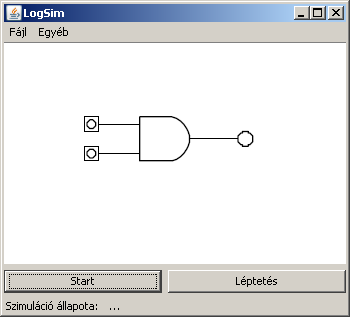
\includegraphics[width=3.64in]{chapters/chapter11/screenshots/felulet.png}
\caption{Főablak}
\label{fig:main}
\end{center}
\end{figure}

\begin{figure}[H]
\begin{center}
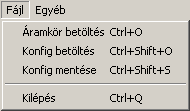
\includegraphics[width=1.98in]{chapters/chapter11/screenshots/menus1.png}
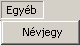
\includegraphics[width=1.479in]{chapters/chapter11/screenshots/menus2.png}
\caption{Fájl és az Egyéb menü almenüi}
\label{fig:menus}
\end{center}
\end{figure}

\begin{figure}[H]
\begin{center}
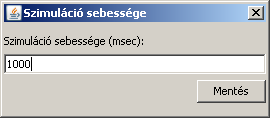
\includegraphics[width=2.8125in]{chapters/chapter11/screenshots/szimseb.png}
\caption{Szimuláció sebességének beállítása}
\label{fig:szimseb}
\end{center}
\end{figure}

\begin{figure}[H]
\begin{center}
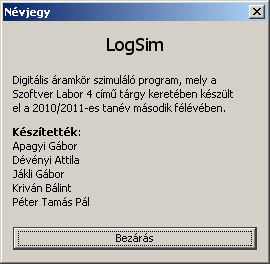
\includegraphics[width=2.8125in]{chapters/chapter11/screenshots/about.png}
\caption{Névjegy}
\label{fig:about}
\end{center}
\end{figure}

\begin{figure}[H]
\begin{center}
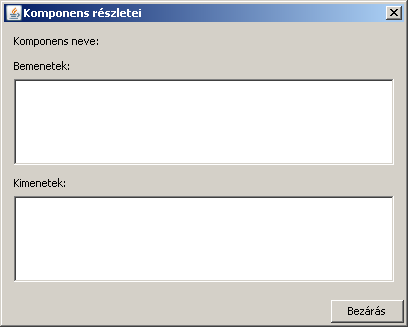
\includegraphics[width=4.25in]{chapters/chapter11/screenshots/details.png}
\caption{Komponens részletei}
\label{fig:gui_szimseb}
\end{center}
\end{figure}

\begin{figure}[H]
\begin{center}
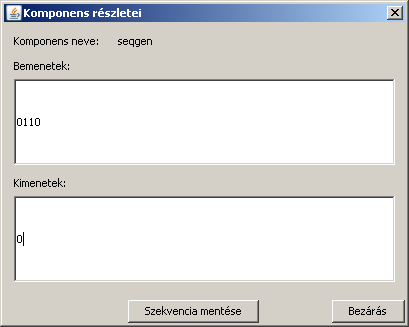
\includegraphics[width=4.25in]{chapters/chapter11/screenshots/details_sg.png}
\caption{Szekvencia generátor beállítása}
\label{fig:gui_szimseb}
\end{center}
\end{figure}


\section{A grafikus rendszer architektúrája}
\comment{A felület működésének elve, a grafikus rendszer architektúrája (struktúra diagramok). A struktúra diagramokon a prototípus azon és csak azon osztályainak is szerepelnie kell, amelyekhez a grafikus felületet létrehozó osztályok kapcsolódnak.}

\subsection{A felület működési elve}
\comment{Le kell írni, hogy a grafikai megjelenésért felelős osztályok, objektumok hogyan kapcsolódnak a meglevő rendszerhez, a megjelenítés során mi volt az alapelv. Törekedni kell az MVC megvalósításra. Alapelvek lehetnek: \textbf{push} alapú: a modell értesíti a felületet, hogy változott; \textbf{pull} alapú: a felület kérdezi le a modellt, hogy változott-e; \textbf{kevert}: a kettő kombinációja.}

Az általunk elkészített grafikus felület "pull" típusú, vagyis a grafikus rendszer kérdezi le a modell objektumoktól az aktuális állapotukat.
Azokhoz a modellobjektumokhoz, melyeket megjelenítünk, elkészítettünk egy-egy wrapper osztályt, mely a megjelenítésért és a megjelenítéshez szükséges információk tárolásáért felel. 
Az áramkört egy JPanel-ra rajzoljuk, mely biztosítja számunkra, hogy az elhelyezhető legyen bármilyen ablakon. Áramkör újrarajzoláskor, az eltárolt objektumok egyenkét rajzolják ki magukat az előzöleg megadott koordináták alapján.
Bármilyen felhasználói interakciónál, melynél változhat az áramkör állapota, az egész áramkört újrarajzoljuk, biztosítva ezzel, hogy a kirajzolt áramkör mindig az aktuális állapotban legyen megjelenítve.


\subsection{A felület osztály-struktúrája}

\begin{figure}[H]
\begin{center}
\includegraphics*[width=17cm]{chapters/chapter11/pdfs/class.pdf}
\caption{Statikus struktúra nézet}
\label{fig:class_diagram}
\end{center}
\end{figure}

\section{A grafikus objektumok felsorolása}

\subsection{Config}
\begin{itemize}
\item Felelősség\\
Konfigurációs fájlok kezelése, azok írása az áramkör alapján, illetve azok betöltése  az áramkörbe.
\item Ősosztályok\ Object $\rightarrow{}$ Config.
\item Interfészek (nincs)
\item Attribútumok $\ $
\begin{itemize}
	\item[] \texttt{$-$ Circuit circuit} Áramkör, aminek mentjük a dolgait
	\item[] \texttt{$-$ Pattern \underline{sourceComponentPattern}} Regex kifejezés az illesztéshez (beolvasásnál)
\end{itemize}
\item Metódusok$\ $
\begin{itemize}
	\item[] \texttt{$+$ Config(Circuit circuit)}: Példány létrehozása az áramkörhöz.
	\item[] \texttt{$+$ int load(File file)}: Betölti egy fájlból a kapcsolók illetve jelgenerátorok konfigurációját
	\item[] \texttt{$+$ int save(File file)}: Elmenti a kapcsolók illetve jelgenerátorok aktuális állapotát egy fájlba
\end{itemize}
\end{itemize}

\subsection{Controller}
Interfész.
\begin{itemize}
\item Felelősség\\
Kontroller interfész.
\item Ősosztályok\ Controller.
\item Interfészek (nincs)
\item Metódusok$\ $
\begin{itemize}
	\item[] \texttt{$+$ void run(BufferedReader input)}: Vezérlés elindítása adott bemenetről.
\end{itemize}
\end{itemize}

\subsection{Parser}
\begin{itemize}
\item Felelősség\\
Áramkör értelmező objektum, feladata, hogy a paraméterként átadott, illetve  fájlban elhelyezett komponenseket értelmezze, a kapcsolatokat feltérképezze,  elvégezze az összeköttetéseket, és ezáltal felépítse az áramkört.
\item Ősosztályok\ Object $\rightarrow{}$ Parser.
\item Interfészek (nincs)
\item Attribútumok $\ $
\begin{itemize}
	\item[] \texttt{$-$ Circuit circuit} A leíróból létrehozott áramkör.
	\item[] \texttt{$-$ Pattern \underline{componentPattern}} Regex minta egy komponens-sor feldolgozásához
	\item[] \texttt{$-$ Pattern \underline{compositeEndPattern}} Regex minta egy kompozit véghez
	\item[] \texttt{$-$ Map composites} Komponensek listája név szerint.
	\item[] \texttt{$-$ Pattern \underline{compositeStartPattern}} Regex minta egy kompozit kezdethez
	\item[] \texttt{$-$ Map parameters} Kompozitokban lévő komponensek paraméter listája.
\end{itemize}
\item Metódusok$\ $
\begin{itemize}
	\item[] \texttt{$+$ Parser()}: 
 % TODO
	\item[] \texttt{$-$ void addComponentsToComposite(Composite composite, List lines, String[] inputs, String[] outputs)}: Komponens hozzáadása a kompozithoz
	\item[] \texttt{$-$ void parse(BufferedReader br)}: Bementről feldolgozás
	\item[] \texttt{$+$ Circuit parse(File file)}: Létrehoz egy áramkört a megadott fájlból
	\item[] \texttt{$-$ AbstractComponent parseComponentFromLine(Matcher matcher, Composite composite)}: Egy komponens-sor feldolgozása a fájlban
\end{itemize}
\end{itemize}

\subsection{Proto}
\begin{itemize}
\item Felelősség\\
Prototípus vezérlő osztálya.
\item Ősosztályok\ Object $\rightarrow{}$ Proto.
\item Interfészek Controller.
\item Attribútumok $\ $
\begin{itemize}
	\item[] \texttt{$-$ Circuit c} Áramkör
	\item[] \texttt{$-$ Config config} Konfiguráció menedzselése
	\item[] \texttt{$-$ Simulation s} Szimuláció
	\item[] \texttt{$-$ Viewable view} Megjelenítő
\end{itemize}
\item Metódusok$\ $
\begin{itemize}
	\item[] \texttt{$+$ Proto()}: 
 % TODO
	\item[] \texttt{$-$ void eval(String s)}: Parancs értelmezése
	\item[] \texttt{$+$ static void main(String[] args)}: Program belépési pontja.
	\item[] \texttt{$+$ void run(BufferedReader input)}: Felhasználó parancsait olvassa
\end{itemize}
\end{itemize}

\subsection{View}
\begin{itemize}
\item Felelősség\\
Egy konkrét kimeneti implementáció, mely OutputStreamWriter-be ír ki,  így a konzolos megjelenítés és fájlba írás megoldott.
\item Ősosztályok\ Object $\rightarrow{}$ View.
\item Interfészek Viewable.
\item Attribútumok $\ $
\begin{itemize}
	\item[] \texttt{$-$ Controller controller} Kontroller
	\item[] \texttt{$-$ PrintWriter out} Kimeneti adatfolyam, ide írunk.
\end{itemize}
\item Metódusok$\ $
\begin{itemize}
	\item[] \texttt{$+$ View(Controller c, OutputStreamWriter out)}: Létehozzuk a Viewt egy kontrollerrel és a kimenettel, ide fog menni a kimenet.
	\item[] \texttt{$+$ void newline()}: Új sor a kimeneten
	\item[] \texttt{$+$ void writeDetails(AbstractComponent ac)}: Kiírunk egy komponenst (be és kimenetek)
	\item[] \texttt{$+$ void writeLedValue(Led led)}: Kiírja a led értékét
	\item[] \texttt{$+$ void writeLoadFailed()}: Kiírjuk, hogy a betöltés sikertelen
	\item[] \texttt{$+$ void writeLoadSuccessful()}: Kiírjuk, hogy betöltés sikeres
	\item[] \texttt{$+$ void writeSaveFailed()}: Kiírjuk, hogy a config fájl sikertelen
	\item[] \texttt{$+$ void writeSaveSuccessful()}: Kiírjuk, hogy a config fájl mentés sikeres
	\item[] \texttt{$+$ void writeScopeDetails(Scope ac)}: Kiírunk egy scope-ot
	\item[] \texttt{$+$ void writeScopeValues(Scope scope)}: Kiírja a scope által tárolt értékeket
	\item[] \texttt{$+$ void writeSequenceGenerator(SequenceGenerator sg)}: Szekvenciagenerátor szekvenciájának kiírása
	\item[] \texttt{$+$ void writeSequenceGeneratorSequence(SequenceGenerator sg)}: Kiírja a jelgenerátor szekvenciáját
	\item[] \texttt{$+$ void writeSequenceGeneratorValue(SequenceGenerator sg)}: Kiírja a jelgenerátor éppen kiadott értékét
	\item[] \texttt{$+$ void writeSevenSegmentDisplayValues(SevenSegmentDisplay seg)}: Kiírja a 7-szegmentes kijelző szegmenseit.
	\item[] \texttt{$+$ void writeSimulationFailed()}: Kiírjuk, hogy a szimuláció sikertelen
	\item[] \texttt{$+$ void writeSimulationSuccessful()}: Kiírjuk, hogy a szimuláció sikeres
	\item[] \texttt{$+$ void writeToggleValue(Toggle sc)}: Kiírja a kapcsoló állapotát
\end{itemize}
\end{itemize}

\subsection{Viewable}
Interfész.
\begin{itemize}
\item Felelősség\\
A kimenet interfésze.
\item Ősosztályok\ Viewable.
\item Interfészek (nincs)
\item Metódusok$\ $
\begin{itemize}
	\item[] \texttt{$+$ void newline()}: Új sor a kimeneten
	\item[] \texttt{$+$ void writeDetails(AbstractComponent ac)}: Kiírunk egy komponenst (be és kimenetek)
	\item[] \texttt{$+$ void writeLedValue(Led led)}: Kiírja a led értékét
	\item[] \texttt{$+$ void writeLoadFailed()}: Kiírjuk, hogy a betöltés sikertelen
	\item[] \texttt{$+$ void writeLoadSuccessful()}: Kiírjuk, hogy betöltés sikeres
	\item[] \texttt{$+$ void writeSaveFailed()}: Kiírjuk, hogy a config fájl sikertelen
	\item[] \texttt{$+$ void writeSaveSuccessful()}: Kiírjuk, hogy a config fájl mentés sikeres
	\item[] \texttt{$+$ void writeScopeDetails(Scope scope)}: Kiírunk egy scope-ot
	\item[] \texttt{$+$ void writeScopeValues(Scope scope)}: Kiírja a scope által tárolt értékeket
	\item[] \texttt{$+$ void writeSequenceGenerator(SequenceGenerator sg)}: Szekvenciagenerátor szekvenciájának kiírása
	\item[] \texttt{$+$ void writeSequenceGeneratorSequence(SequenceGenerator sg)}: Kiírja a jelgenerátor szekvenciáját
	\item[] \texttt{$+$ void writeSequenceGeneratorValue(SequenceGenerator sg)}: Kiírja a jelgenerátor éppen kiadott értékét
	\item[] \texttt{$+$ void writeSevenSegmentDisplayValues(SevenSegmentDisplay seg)}: Kiírja a 7-szegmentes kijelző szegmenseit.
	\item[] \texttt{$+$ void writeSimulationFailed()}: Kiírjuk, hogy a szimuláció sikertelen
	\item[] \texttt{$+$ void writeSimulationSuccessful()}: Kiírjuk, hogy a szimuláció sikeres
	\item[] \texttt{$+$ void writeToggleValue(Toggle toggle)}: Kiírja a kapcsoló állapotát
\end{itemize}
\end{itemize}


\subsection{Circuit}
\begin{itemize}
\item Felelősség\\
Áramkört reprezentáló osztály, igazából egy kompozit. Felelőssége megegyzik a kompozitéval.
\item Ősosztályok\ Object $\rightarrow{}$ AbstractComponent $\rightarrow{}$ Composite $\rightarrow{}$ Circuit.
\item Interfészek (nincs)
\item Attribútumok $\ $
\begin{itemize}
\item (nincs)
\end{itemize}
\item Metódusok$\ $
\begin{itemize}
	\item[] \texttt{$+$ Circuit()}: 
 % TODO
\end{itemize}
\end{itemize}

\subsection{Simulation}
\begin{itemize}
\item Felelősség\\
Egy szimulációt reprezentáló objektum.  Utasítja az áramkört, hogy értékelje ki magát. Ha az áramkör azt jelzi magáról,  hogy nincs stacionárius állapota akkor jelezzük a felhasználónak.
\item Ősosztályok\ Object $\rightarrow{}$ Simulation.
\item Interfészek (nincs)
\item Attribútumok $\ $
\begin{itemize}
	\item[] \texttt{$\#$ Circuit circuit} Szimulált áramkör
\end{itemize}
\item Metódusok$\ $
\begin{itemize}
	\item[] \texttt{$+$ Simulation()}: 
 % TODO
	\item[] \texttt{$+$ void setCircuit(Circuit circuit)}: Szimulált áramkör beállítása
	\item[] \texttt{$+$ boolean start()}: Egy adott bemeneti kombinációkra kiértékeli a hálózatot.
\end{itemize}
\end{itemize}

\subsection{Value}
\begin{itemize}
\item Felelősség\\
Az áramkörben előfordulható értéket reprezentál.
\item Ősosztályok\ Object $\rightarrow{}$ Enum $\rightarrow{}$ Value.
\item Interfészek (nincs)
\item Attribútumok $\ $
\begin{itemize}
	\item[] \texttt{$+$ final Value \underline{FALSE}} 
 % TODO
	\item[] \texttt{$+$ final Value \underline{TRUE}} 
 % TODO
\end{itemize}
\item Metódusok$\ $
\begin{itemize}
	\item[] \texttt{$-$ Value()}: 
 % TODO
	\item[] \texttt{$+$ Value invert()}: Érték invertálása
	\item[] \texttt{$+$ static Value valueOf(String name)}: 
 % TODO
	\item[] \texttt{$+$ static Value[] values()}: 
 % TODO
\end{itemize}
\end{itemize}


\subsection{AbstractComponent}
Absztrakt osztály.
\begin{itemize}
\item Felelősség\\
Egy komponens absztrakt megvalósítása, ebből származik az összes többi  komponens. A közös logikát valósítja meg. A gyakran használt dolgokra  ad alapértelmezett implementációt (kimenetekre és bemenetekre kötés, kiértékelés stb.)
\item Ősosztályok\ Object $\rightarrow{}$ AbstractComponent.
\item Interfészek (nincs)
\item Attribútumok $\ $
\begin{itemize}
	\item[] \texttt{$-$ boolean changed} Változott-e a komponens kimenete
	\item[] \texttt{$\#$ Wire[] inputs} Bemenetekre kötött vezetékek
	\item[] \texttt{$\#$ String name} Komponens neve
	\item[] \texttt{$\#$ Wire[] outputs} Kimenetekre kötött vezetékek
\end{itemize}
\item Metódusok$\ $
\begin{itemize}
	\item[] \texttt{$\#$ AbstractComponent(String name, int inputCount, int outputCount)}: Konstruktor
	\item[] \texttt{$+$ void addTo(Composite composite)}: Komponens hozzáadása az áramkörhöz
	\item[] \texttt{$+$ abstract AbstractComponent copy(String newName)}: Lemásoljuk a komponenst.
	\item[] \texttt{$+$ void evaluate()}: Komponens kimeneti lábain lévő vezetékeken lévő értékek újraszámolása  a bemenetek alapján.
	\item[] \texttt{$\#$ Value getInput(int inputPin)}: Lekérjük egy adott bemenetre kötött értéket
	\item[] \texttt{$+$ int getInputsCount()}: Bemeneti lábak száma
	\item[] \texttt{$+$ Wire getInputWire(int inputPin)}: Lekérünk egy bemeneti lábon lévő vezetéket
	\item[] \texttt{$+$ String getName()}: Komponens nevének lekérése.
	\item[] \texttt{$+$ int getOutputsCount()}: Kimeneti lábak száma
	\item[] \texttt{$+$ Wire getOutputWire(int outputPin)}: Lekérünk egy kimeneti lábon lévő vezetéket
	\item[] \texttt{$+$ boolean isChanged()}: Visszaadja, hogy a komponensünk kimeneti értéke változott-e a kiértékelés során
	\item[] \texttt{$\#$ abstract void onEvaluation()}: Ebben a metódusban kell implementálni az alkatrész logikáját, vagyis  az adott bemenet(ek) függvényében mit kell kiadnia a kimenet(ek)re.
	\item[] \texttt{$+$ void setInput(int inputPin, Wire wire)}: Beállítunk egy bemenetet
	\item[] \texttt{$+$ void setOutput(int outputPin, Wire wire)}: Beállítunk egy kimenetet
	\item[] \texttt{$+$ void writeTo(Viewable view)}: Komponens kiírása a viewra.
	\item[] \texttt{$+$ void writeValueTo(Viewable view)}: Kiírja az értékét a viewra (csak kijelző és forrásra!)
\end{itemize}
\end{itemize}

\subsection{Composite}
\begin{itemize}
\item Felelősség\\
Kompozit elem leírása, kiértékelésnél a tartalmazott komponenseket kiértékeli, lépteti  a jelgenerátorokat stb. Ha nem áll be stacionárius állapotba a kiértékelésnél, akkor ezt jelzi kifelé.
\item Ősosztályok\ Object $\rightarrow{}$ AbstractComponent $\rightarrow{}$ Composite.
\item Interfészek (nincs)
\item Attribútumok $\ $
\begin{itemize}
	\item[] \texttt{$-$ Map components} Komponensek listája
	\item[] \texttt{$-$ List composites} Kompozit típusú komponensek listája
	\item[] \texttt{$-$ final int \underline{cycleLimit}} Max. ciklusok száma
	\item[] \texttt{$-$ List displays} Megjelenítő típusú komponensek listája (pl. led)
	\item[] \texttt{$-$ List flipFlops} Flipflopok listája
	\item[] \texttt{$-$ List generators} Jelgenerátorok listája
	\item[] \texttt{$-$ Node[] inputNodes} Bemeneti csomópontok
	\item[] \texttt{$-$ Pattern \underline{inputPattern}} Regex minta egy komponens bemeneteinek a feldolgozásához
	\item[] \texttt{$-$ Node[] outputNodes} Kimeneti csomópontok
	\item[] \texttt{$-$ List scopes} Oszcillátor típusú komponensek listája
	\item[] \texttt{$-$ List sources} Jelforrás típusú komponensek listája (pl. kapcsoló)
	\item[] \texttt{$-$ String type} Kompozit típusa
\end{itemize}
\item Metódusok$\ $
\begin{itemize}
	\item[] \texttt{$+$ Composite(String type, String name, int inputCount, int outputCount)}: Adott típusú és nevű komponens létrehozása a megfelelő lábszámmal.
	\item[] \texttt{$+$ void add(AbstractComponent c)}: Általános típusú komponens hozzáadása
	\item[] \texttt{$+$ void add(Composite c)}: Kompozit típusú komponens hozzáadása
	\item[] \texttt{$+$ void add(DisplayComponent dc)}: Kijelző típusú komponens hozzáadása
	\item[] \texttt{$+$ void add(FlipFlop ff)}: Flipflop komponens hozzáadása
	\item[] \texttt{$+$ void add(Scope scope)}: Oszcillátor típusú komponens hozzáadása
	\item[] \texttt{$+$ void add(SequenceGenerator sg)}: Jelgenerátor komponens hozzáadása
	\item[] \texttt{$+$ void add(SourceComponent sc)}: Jelforrás típusú komponens hozzáadása
	\item[] \texttt{$+$ void addTo(Composite composite)}: Kompozit hozzáadása kompozithoz.
	\item[] \texttt{$-$ void commitFlipFlops()}: A flipflopok jelenlegi kimenetét elmentjük belső állapotnak, és az órajel  bemenetén lévő értéket pedig eltároljuk az éldetektálás érdekében.
	\item[] \texttt{$-$ void commitScopes()}: Oszcilloszkópok véglegesítése
	\item[] \texttt{$+$ void connectComponents(Map connections, String[] inputs, String[] outputs)}: Komponensek összekötése
	\item[] \texttt{$+$ Composite copy(String variableName)}: Kompozit lemásolása (példányosításnál használjuk.)
	\item[] \texttt{$+$ AbstractComponent getComponentByName(String name)}: Komponens lekérése a neve alapján (delegálja a kérést, ha kell).
	\item[] \texttt{$+$ Collection getComponents()}: Összes tartalmazott komponens listája
	\item[] \texttt{$+$ List getDisplayComponents()}: Megjelenítők listája
	\item[] \texttt{$+$ List getSourceComponents()}: Jelforrások listája
	\item[] \texttt{$+$ List getStepGenerators()}: Jelgenerátorok listája
	\item[] \texttt{$\#$ void onEvaluation()}: Kiértékelési ciklus
	\item[] \texttt{$+$ void setInput(int inputPin, Wire wire)}: Bemenet beállítása
	\item[] \texttt{$+$ void setOutput(int outputPin, Wire wire)}: Kimenet beállítása
	\item[] \texttt{$-$ void stepGenerators()}: Jelgenerátorok léptetése
\end{itemize}
\end{itemize}

\subsection{DisplayComponent}
Absztrakt osztály.
\begin{itemize}
\item Felelősség\\
Megjelenítő típusú komponenst reprezentál. Tőle származnak a megjelenítők (pl. led).
\item Ősosztályok\ Object $\rightarrow{}$ AbstractComponent $\rightarrow{}$ DisplayComponent.
\item Interfészek (nincs)
\item Attribútumok $\ $
\begin{itemize}
\item (nincs)
\end{itemize}
\item Metódusok$\ $
\begin{itemize}
	\item[] \texttt{$\#$ DisplayComponent(String name, int inputCount)}: Konstruktor. Nem lesz kimenete.
	\item[] \texttt{$+$ void addTo(Composite composite)}: Hozzáadás kompozithoz
\end{itemize}
\end{itemize}

\subsection{FlipFlop}
Absztrakt osztály.
\begin{itemize}
\item Felelősség\\
Flipflopok ősosztálya, minden flipflop 1. bemenete az órajel!
\item Ősosztályok\ Object $\rightarrow{}$ AbstractComponent $\rightarrow{}$ FlipFlop.
\item Interfészek (nincs)
\item Attribútumok $\ $
\begin{itemize}
	\item[] \texttt{$\#$ Value clk} Előző érvényes órajel, ettől és a kiértékelés pillanatában lévő órajel értékétől  függően észlelhetjük, hogy felfutó él van-e vagy sem.
	\item[] \texttt{$\#$ final int \underline{CLK}} Fixen az 1. bemenet az órajel
	\item[] \texttt{$\#$ Value q} Belső memóriája, ami a kimenetén megjelenik, órajel felfutó élénél változhat az állapota.
\end{itemize}
\item Metódusok$\ $
\begin{itemize}
	\item[] \texttt{$+$ FlipFlop(String name, int inputCount)}: 
 % TODO
	\item[] \texttt{$+$ void addTo(Composite composite)}: Hozzáadás kompozithoz
	\item[] \texttt{$+$ void commit()}: Véglegesítés
	\item[] \texttt{$+$ boolean isActive()}: Számolhat-e az FF? Ezt hívja meg az FF-ek onEvaluation() metódusa, mielőtt  bármit is csinálnának.
	\item[] \texttt{$\#$ abstract void onCommit()}: Kimenetre értékadás a logika elvégzése után.
	\item[] \texttt{$\#$ void onEvaluation()}: Nem csinálunk semmit, majd csak commit()-nál.
\end{itemize}
\end{itemize}

\subsection{SourceComponent}
Absztrakt osztály.
\begin{itemize}
\item Felelősség\\
Jelforrás típusú komponenst reprezentál. Tőle származnak a jelforrások (pl. toggle).
\item Ősosztályok\ Object $\rightarrow{}$ AbstractComponent $\rightarrow{}$ SourceComponent.
\item Interfészek (nincs)
\item Attribútumok $\ $
\begin{itemize}
\item (nincs)
\end{itemize}
\item Metódusok$\ $
\begin{itemize}
	\item[] \texttt{$\#$ SourceComponent(String name)}: Konstruktor. Nincs bemenete és egy kimenete van
	\item[] \texttt{$+$ void addTo(Composite composite)}: Hozzáadás kompozithoz.
	\item[] \texttt{$+$ abstract Value[] getValues()}: Lekérhetjük a jelforrás értékeit, hogy el tudjuk menteni.
	\item[] \texttt{$+$ abstract void reset()}: Jelforrás nullázása
	\item[] \texttt{$+$ abstract void setValues(Value[] values)}: Beállítjuk a jelforrás értékét. Kapcsoló esetén csak 1 elemű tömb  adható paraméterként!
\end{itemize}
\end{itemize}

\subsection{Wire}
\begin{itemize}
\item Felelősség\\
Vezeték osztály. Két komponens-lábat köt össze. A rajta lévő érték lekérdezhető  és beállítható.
\item Ősosztályok\ Object $\rightarrow{}$ Wire.
\item Interfészek (nincs)
\item Attribútumok $\ $
\begin{itemize}
	\item[] \texttt{$-$ Value value} Vezetéken lévő érték
\end{itemize}
\item Metódusok$\ $
\begin{itemize}
	\item[] \texttt{$+$ Wire()}: 
 % TODO
	\item[] \texttt{$+$ Value getValue()}: Vezeték értékének lekérése
	\item[] \texttt{$+$ void setValue(Value value)}: Vezeték értékének beállítása
\end{itemize}
\end{itemize}


\subsection{AndGate}
\begin{itemize}
\item Felelősség\\
ÉS kapu, az áramkör egyik alapeleme. Bemeneteire kötött komponensek  kiértékelését kezdeményezi, s a kapott értékek logikai ÉS kapcsolatát  valósítja meg, amit a kimenetén kiad.
\item Ősosztályok\ Object $\rightarrow{}$ AbstractComponent $\rightarrow{}$ AndGate.
\item Interfészek (nincs)
\item Attribútumok $\ $
\begin{itemize}
\item (nincs)
\end{itemize}
\item Metódusok$\ $
\begin{itemize}
	\item[] \texttt{$+$ AndGate(int pinsCount, String name)}: 
 % TODO
	\item[] \texttt{$+$ AndGate copy(String newName)}: 
 % TODO
	\item[] \texttt{$\#$ void onEvaluation()}: 
 % TODO
\end{itemize}
\end{itemize}

\subsection{FlipFlopD}
\begin{itemize}
\item Felelősség\\
D flipflop, mely felfutó órajelnél beírja a belső memóriába az adatbemeneten (D)  lévő értéket.
\item Ősosztályok\ Object $\rightarrow{}$ AbstractComponent $\rightarrow{}$ FlipFlop $\rightarrow{}$ FlipFlopD.
\item Interfészek (nincs)
\item Attribútumok $\ $
\begin{itemize}
	\item[] \texttt{$-$ final int \underline{D}} D bemenet lábának a száma.
\end{itemize}
\item Metódusok$\ $
\begin{itemize}
	\item[] \texttt{$+$ FlipFlopD(String name)}: 
 % TODO
	\item[] \texttt{$+$ FlipFlopD copy(String newName)}: 
 % TODO
	\item[] \texttt{$\#$ void onEvaluation()}: 
 % TODO
\end{itemize}
\end{itemize}

\subsection{FlipFlopJK}
\begin{itemize}
\item Felelősség\\
JK flipflop, mely a belső memóriáját a Követelmények résznél leírt módon  a J és K bemenetektől függően változtatja.
\item Ősosztályok\ Object $\rightarrow{}$ AbstractComponent $\rightarrow{}$ FlipFlop $\rightarrow{}$ FlipFlopJK.
\item Interfészek (nincs)
\item Attribútumok $\ $
\begin{itemize}
	\item[] \texttt{$-$ final int \underline{J}} J bemenet lábának a száma
	\item[] \texttt{$-$ final int \underline{K}} K bemenet lábának a száma
\end{itemize}
\item Metódusok$\ $
\begin{itemize}
	\item[] \texttt{$+$ FlipFlopJK(String name)}: 
 % TODO
	\item[] \texttt{$+$ FlipFlopJK copy(String newName)}: 
 % TODO
	\item[] \texttt{$\#$ void onEvaluation()}: 
 % TODO
\end{itemize}
\end{itemize}

\subsection{Gnd}
\begin{itemize}
\item Felelősség\\
A "föld" komponens, mely állandóan a hamis értéket adja ki. Nincs bemenete.
\item Ősosztályok\ Object $\rightarrow{}$ AbstractComponent $\rightarrow{}$ Gnd.
\item Interfészek (nincs)
\item Attribútumok $\ $
\begin{itemize}
\item (nincs)
\end{itemize}
\item Metódusok$\ $
\begin{itemize}
	\item[] \texttt{$+$ Gnd(String name)}: 
 % TODO
	\item[] \texttt{$+$ AbstractComponent copy(String newName)}: 
 % TODO
	\item[] \texttt{$\#$ void onEvaluation()}: 
 % TODO
\end{itemize}
\end{itemize}

\subsection{Inverter}
\begin{itemize}
\item Felelősség\\
Inverter alkatrész, mely invertálva adja ki a kimenetén a bemenetén  érkező jelet.
\item Ősosztályok\ Object $\rightarrow{}$ AbstractComponent $\rightarrow{}$ Inverter.
\item Interfészek (nincs)
\item Attribútumok $\ $
\begin{itemize}
\item (nincs)
\end{itemize}
\item Metódusok$\ $
\begin{itemize}
	\item[] \texttt{$+$ Inverter(String name)}: Konstruktor. 1 bemenet és 1 kimenet
	\item[] \texttt{$+$ AbstractComponent copy(String name)}: 
 % TODO
	\item[] \texttt{$\#$ void onEvaluation()}: 
 % TODO
\end{itemize}
\end{itemize}

\subsection{Led}
\begin{itemize}
\item Felelősség\\
Egy LED-et reprezentál, mely világít, ha bemenetén igaz érték van.
\item Ősosztályok\ Object $\rightarrow{}$ AbstractComponent $\rightarrow{}$ DisplayComponent $\rightarrow{}$ Led.
\item Interfészek (nincs)
\item Attribútumok $\ $
\begin{itemize}
\item (nincs)
\end{itemize}
\item Metódusok$\ $
\begin{itemize}
	\item[] \texttt{$+$ Led(String name)}: Konstruktor. 1 bemenetű megjelenítő
	\item[] \texttt{$+$ Led copy(String name)}: 
 % TODO
	\item[] \texttt{$+$ Value getValue()}: Visszaadja a led értékét
	\item[] \texttt{$\#$ void onEvaluation()}: 
 % TODO
	\item[] \texttt{$+$ void writeValueTo(Viewable view)}: 
 % TODO
\end{itemize}
\end{itemize}

\subsection{Mpx}
\begin{itemize}
\item Felelősség\\
4-1-es multiplexer, melynek a bemeneti lábak sorrendje a következő:  D0, D1, D2, D3, S0, S1. Ahol Dx az adatbemenetek, Sy a kiválasztóbemenetek.  Kimenetén a kiválasztóbemenetektől függően valamelyik adatbemenet kerül kiadásra.
\item Ősosztályok\ Object $\rightarrow{}$ AbstractComponent $\rightarrow{}$ Mpx.
\item Interfészek (nincs)
\item Attribútumok $\ $
\begin{itemize}
	\item[] \texttt{$-$ final int \underline{DATA0}} 
 % TODO
	\item[] \texttt{$-$ final int \underline{DATA1}} 
 % TODO
	\item[] \texttt{$-$ final int \underline{DATA2}} 
 % TODO
	\item[] \texttt{$-$ final int \underline{DATA3}} 
 % TODO
	\item[] \texttt{$-$ final int \underline{SEL0}} 
 % TODO
	\item[] \texttt{$-$ final int \underline{SEL1}} 
 % TODO
\end{itemize}
\item Metódusok$\ $
\begin{itemize}
	\item[] \texttt{$+$ Mpx(String name)}: 
 % TODO
	\item[] \texttt{$+$ Mpx copy(String newName)}: 
 % TODO
	\item[] \texttt{$\#$ void onEvaluation()}: 
 % TODO
\end{itemize}
\end{itemize}

\subsection{Node}
\begin{itemize}
\item Felelősség\\
Csomópont elem. Az egyetlen bemenetére kötött értéket kiadja az összes kimeneti lábán.
\item Ősosztályok\ Object $\rightarrow{}$ AbstractComponent $\rightarrow{}$ Node.
\item Interfészek (nincs)
\item Attribútumok $\ $
\begin{itemize}
\item (nincs)
\end{itemize}
\item Metódusok$\ $
\begin{itemize}
	\item[] \texttt{$+$ Node(int outputPinsCount, String name)}: Konstruktor. 1 bemenete van
	\item[] \texttt{$+$ AbstractComponent copy(String name)}: 
 % TODO
	\item[] \texttt{$\#$ void onEvaluation()}: 
 % TODO
\end{itemize}
\end{itemize}

\subsection{OrGate}
\begin{itemize}
\item Felelősség\\
VAGY kapu, az áramkör egyik alapeleme. Bemenetein lévő értékek logikai VAGY kapcsolatát  valósítja meg, amit a kimenetén kiad.
\item Ősosztályok\ Object $\rightarrow{}$ AbstractComponent $\rightarrow{}$ OrGate.
\item Interfészek (nincs)
\item Attribútumok $\ $
\begin{itemize}
\item (nincs)
\end{itemize}
\item Metódusok$\ $
\begin{itemize}
	\item[] \texttt{$+$ OrGate(int inputPinsCount, String name)}: Konstruktor. 1 kimenete van
	\item[] \texttt{$+$ AbstractComponent copy(String name)}: 
 % TODO
	\item[] \texttt{$\#$ void onEvaluation()}: 
 % TODO
\end{itemize}
\end{itemize}

\subsection{Scope}
\begin{itemize}
\item Felelősség\\
Egy oszcilloszkópot reprezentál. Eltárolt értékek egy sorba kerülnek bele, mely fix méretű.
\item Ősosztályok\ Object $\rightarrow{}$ AbstractComponent $\rightarrow{}$ DisplayComponent $\rightarrow{}$ Led $\rightarrow{}$ Scope.
\item Interfészek (nincs)
\item Attribútumok $\ $
\begin{itemize}
	\item[] \texttt{$-$ Queue memory} Eltárolt értékek sora.
	\item[] \texttt{$-$ int size} Eltárolható értékek száma.
\end{itemize}
\item Metódusok$\ $
\begin{itemize}
	\item[] \texttt{$+$ Scope(int size, String name)}: Konstruktor. 1 bemenetű megjelenítő
	\item[] \texttt{$+$ void addTo(Composite composite)}: Hozzáadás kompozithoz.
	\item[] \texttt{$+$ void commit()}: Eltároljuk az értéket a memóriában
	\item[] \texttt{$+$ Scope copy(String name)}: 
 % TODO
	\item[] \texttt{$+$ Value[] getValues()}: Visszaadja az eddig eltárolt értékeket
	\item[] \texttt{$\#$ void onEvaluation()}: 
 % TODO
	\item[] \texttt{$+$ void writeTo(Viewable view)}: Komponens kiírása a viewra.
	\item[] \texttt{$+$ void writeValueTo(Viewable view)}: Érték kiírása a kimenetre.
\end{itemize}
\end{itemize}

\subsection{SequenceGenerator}
\begin{itemize}
\item Felelősség\\
Jelgenerátort reprezentál, amely a beállított bitsorozatot adja ki.  Alapértelmezetten (amíg a felhasználó nem állítja be, vagy tölt be másikat) a 0,1-es  szekvenciát tárolja.
\item Ősosztályok\ Object $\rightarrow{}$ AbstractComponent $\rightarrow{}$ SourceComponent $\rightarrow{}$ SequenceGenerator.
\item Interfészek (nincs)
\item Attribútumok $\ $
\begin{itemize}
	\item[] \texttt{$-$ int index} Bitsorozat egy indexe, ez határozza meg, hogy éppen melyik értéket adja ki.
	\item[] \texttt{$-$ Value[] sequence} Tárolt bitsorozat
\end{itemize}
\item Metódusok$\ $
\begin{itemize}
	\item[] \texttt{$+$ SequenceGenerator(String name)}: Konstruktor, ami alapállapotban a 0,1-es szekvenciát állítja be.
	\item[] \texttt{$+$ void addTo(Composite composite)}: Hozzáadás kompozithoz.
	\item[] \texttt{$+$ SequenceGenerator copy(String newName)}: 
 % TODO
	\item[] \texttt{$+$ Value[] getValues()}: Jelgenerátor bitsorozatának lekérdezése
	\item[] \texttt{$\#$ void onEvaluation()}: 
 % TODO
	\item[] \texttt{$+$ void setValues(Value[] values)}: Jelgenerátor bitsorozatának beállítása
	\item[] \texttt{$+$ void step()}: A jelgenerátor lép, a bitsorozat következő elemére ugrik. A következő léptetésig  ez kerül kiadásra a kimeneteken.
	\item[] \texttt{$+$ void writeValueTo(Viewable view)}: Érték kiírása a megjelenítőre
\end{itemize}
\end{itemize}

\subsection{SevenSegmentDisplay}
\begin{itemize}
\item Felelősség\\
7-szegmenses kijelzőt reprezentál, melynek 7 bemenete vezérli a  megfelelő szegmenseket, ezek világítanak, ha az adott bemenetre logikai  igaz van kötve.
\item Ősosztályok\ Object $\rightarrow{}$ AbstractComponent $\rightarrow{}$ DisplayComponent $\rightarrow{}$ SevenSegmentDisplay.
\item Interfészek (nincs)
\item Attribútumok $\ $
\begin{itemize}
\item (nincs)
\end{itemize}
\item Metódusok$\ $
\begin{itemize}
	\item[] \texttt{$+$ SevenSegmentDisplay(String name)}: 
 % TODO
	\item[] \texttt{$+$ AbstractComponent copy(String newName)}: 
 % TODO
	\item[] \texttt{$+$ Value getSegment(int segment)}: Egy szegmens értékének lekérdezése
	\item[] \texttt{$\#$ void onEvaluation()}: 
 % TODO
	\item[] \texttt{$+$ void writeValueTo(Viewable view)}: 
 % TODO
\end{itemize}
\end{itemize}

\subsection{Toggle}
\begin{itemize}
\item Felelősség\\
Kapcsoló jelforrás, melyet a felhasználó szimuláció közben kapcsolgathat.
\item Ősosztályok\ Object $\rightarrow{}$ AbstractComponent $\rightarrow{}$ SourceComponent $\rightarrow{}$ Toggle.
\item Interfészek (nincs)
\item Attribútumok $\ $
\begin{itemize}
	\item[] \texttt{$-$ Value v} Kapcsoló állapota
\end{itemize}
\item Metódusok$\ $
\begin{itemize}
	\item[] \texttt{$+$ Toggle(String name)}: Konstruktor
	\item[] \texttt{$+$ AbstractComponent copy(String name)}: 
 % TODO
	\item[] \texttt{$+$ Value[] getValues()}: Lekérjük a kapcsoló értékét (1 elemű tömb)
	\item[] \texttt{$\#$ void onEvaluation()}: 
 % TODO
	\item[] \texttt{$+$ void setValues(Value[] newValues)}: Kapcsoló állapotának változtatása, csak 1 elemű tömböt kaphat paraméterül.
	\item[] \texttt{$+$ void writeValueTo(Viewable view)}: 
 % TODO
\end{itemize}
\end{itemize}

\subsection{Vcc}
\begin{itemize}
\item Felelősség\\
A tápfeszültés komponens, ami konstans igaz értéket ad. Nincs bemenete.
\item Ősosztályok\ Object $\rightarrow{}$ AbstractComponent $\rightarrow{}$ Vcc.
\item Interfészek (nincs)
\item Attribútumok $\ $
\begin{itemize}
\item (nincs)
\end{itemize}
\item Metódusok$\ $
\begin{itemize}
	\item[] \texttt{$+$ Vcc(String name)}: 
 % TODO
	\item[] \texttt{$+$ AbstractComponent copy(String newName)}: 
 % TODO
	\item[] \texttt{$\#$ void onEvaluation()}: 
 % TODO
\end{itemize}
\end{itemize}


\subsection{CircuitView}
\begin{itemize}
\item Felelősség\\
Áramkört kirajzoló panel.
\item Ősosztályok\ JPanel $\rightarrow{}$ CircuitView.
\item Interfészek MouseListener.
\item Attribútumok $\ $
\begin{itemize}
	\item[] \texttt{$-$ List drawables}: kirajzolandók listája
	\item[] \texttt{$-$ FrameView parent}: főablak
	\item[] \texttt{$-$ Map positions}: kirajzolandók pozíciója
\end{itemize}
\item Metódusok$\ $
\begin{itemize}
	\item[] \texttt{$+$ CircuitView()}: Áramkört kirajzoló panel
	\item[] \texttt{$+$ void mouseClicked(MouseEvent me)}: Egérkattintás kezelő
	\item[] \texttt{$+$ void paint(Graphics g)}: Áramkör kirajzolása
	\item[] \texttt{$+$ void refresh()}: Áramkör újrarajzolása.
	\item[] \texttt{$+$ void setParent(FrameView parent)}: Szülő beállítása
	\item[] \texttt{$+$ void updateDrawables(List drawables, Map coords)}: Kirajzolandó objektumok és koordinátáik beállítása
\end{itemize}
\end{itemize}

\subsection{Drawable}
Interfész.
\begin{itemize}
\item Felelősség\\
Áramköri panelre rajzolható objektum.
\item Ősosztályok\ Drawable.
\item Interfészek (nincs)
\item Metódusok$\ $
\begin{itemize}
	\item[] \texttt{$+$ void draw(Graphics g)}: Kirajzolási logika
	\item[] \texttt{$+$ Dimension getDimension()}: Lekérhetjük az objektumtól a méretét, ha beszélhetünk ilyenről.
	\item[] \texttt{$+$ void onClick(Controller controller)}: Komponensre kapcsolás logikája (visszahívhat a vezérlőre)
\end{itemize}
\end{itemize}

\subsection{Frame}
\begin{itemize}
\item Felelősség\\
Alkalmazás főablaka. Ő tartalmazza a CircuitView-t és a menüsort valamint a gombokat.
\item Ősosztályok\ JFrame $\rightarrow{}$ Frame.
\item Interfészek ActionListener, FrameView.
\item Attribútumok $\ $
\begin{itemize}
	\item[] \texttt{$-$ CircuitView circuitView} 
	\item[] \texttt{$-$ Controller controller}: vezérlő
	\item[] \texttt{$-$ Timer t}: időzítő
\end{itemize}
\item Metódusok$\ $
\begin{itemize}
	\item[] \texttt{$+$ Frame(Controller controller)}: Kontruktor
	\item[] \texttt{$-$ void aboutCloseBtnActionPerformed(ActionEvent evt)}: Névjegy ablak bezárása
	\item[] \texttt{$-$ void aboutMIActionPerformed(ActionEvent evt)}: Névjegy menüpont eseményvezérlője
	\item[] \texttt{$+$ void actionPerformed(ActionEvent e)}: Timer tick eventje
	\item[] \texttt{$-$ void closeDetailedBTNActionPerformed(ActionEvent evt)}: Komponens részletei ablak bezárása
	\item[] \texttt{$+$ void drawCircuit()}: Áramkör kirajzolása
	\item[] \texttt{$-$ void exitMIActionPerformed(ActionEvent evt)}: Kilépés menüpont eseményvezérlője
	\item[] \texttt{$+$ Controller getController()}: Lekérdezhető a vezérlő
	\item[] \texttt{$-$ void loadCircuitMIActionPerformed(ActionEvent evt)}: Áramkör betöltése menüpont eseményvezérlője
	\item[] \texttt{$-$ void loadConfigMIActionPerformed(ActionEvent evt)}: Konfig fájl betöltése menüpont eseményvezérlője
	\item[] \texttt{$+$ void makeItVisible()}: Megjelenítés
	\item[] \texttt{$+$ void onFailedSimulation()}: Áramkör szimulációja nem sikerült
	\item[] \texttt{$+$ void onSuccessfulSimulation()}: Áramkör szimulációja sikeres
	\item[] \texttt{$-$ void saveConfigMIActionPerformed(ActionEvent evt)}: Konfig fájl mentése menüpont eseményvezérlője
	\item[] \texttt{$-$ void saveSeqBTNActionPerformed(ActionEvent evt)}: Új szekvencia elmentése
	\item[] \texttt{$+$ void setDrawables(List drawables, Map positions)}: Megjelenítendő objektumok és koordinátáik átadása a megjelenítőnek
	\item[] \texttt{$+$ void setPeriod(int pt)}: Szimuláció sebességének beállítása
	\item[] \texttt{$+$ void showDetails(AbstractComponent ac)}: Általános komponens részleteinek megjelenítése
	\item[] \texttt{$+$ void showDetails(Scope s)}: Scope részleteinek megjelenítése
	\item[] \texttt{$+$ void showDetails(SequenceGenerator sg)}: Szekvenciagenerátor részleteinek megjelenítése
	\item[] \texttt{$-$ void simSpeedSaveBtnActionPerformed(ActionEvent evt)}: Új sebesség mentése
	\item[] \texttt{$-$ void simulationDelayActionPerformed(ActionEvent evt)}: Szimuláció sebességének beállítására szolgáló ablak megjelenítése
	\item[] \texttt{$-$ void StartStopActionPerformed(ActionEvent evt)}: Szimuláció start/stop
	\item[] \texttt{$-$ void stepBtnActionPerformed(ActionEvent evt)}: Léptetés gomb eseményvezérlője
\end{itemize}
\end{itemize}

\subsection{FrameView}
Interfész.
\begin{itemize}
\item Felelősség\\
Főablak interfésze
\item Ősosztályok\ FrameView.
\item Interfészek (nincs)
\item Metódusok$\ $
\begin{itemize}
	\item[] \texttt{$+$ void drawCircuit()}: Kirajzoljuk az áramkört.
	\item[] \texttt{$+$ Controller getController()}: Lekérdezzük a vezérlőt
	\item[] \texttt{$+$ void makeItVisible()}: Itt kell megadni, hogy a főablak, hogy tehető láthatóvá.
	\item[] \texttt{$+$ void onFailedSimulation()}: Itt adható meg, hogy mi történjen, ha nem stabil az áramkör
	\item[] \texttt{$+$ void onSuccessfulSimulation()}: Itt adható meg, hogy mi történjen, ha sikeres egy szimulációs lépés
	\item[] \texttt{$+$ void setDrawables(List drawables, Map positions)}: Beállítjuk a kirajzolandó objektumokat és azok pozícióját.
	\item[] \texttt{$+$ void setPeriod(int pt)}: Szimuláció sebességének beállítása
	\item[] \texttt{$+$ void showDetails(AbstractComponent ac)}: 
Általános komponens részleteinek megjelenítése
	\item[] \texttt{$+$ void showDetails(Scope s)}: 
Scope részleteinek megjelenítése
	\item[] \texttt{$+$ void showDetails(SequenceGenerator sg)}: 
Szekvenciagenerátor részleteinek megjelenítése
\end{itemize}
\end{itemize}


\subsection{ComponentView}
Absztrakt osztály.
\begin{itemize}
\item Felelősség\\
A kirajzoló wrapper objektumok ősosztálya. Itt irhatjuk le a közös kirajzoló logikákat (pl. kábelek pinjei).
\item Ősosztályok\ Object $\rightarrow{}$ ComponentView.
\item Interfészek Drawable.
\item Attribútumok $\ $
\begin{itemize}
	\item[] \texttt{$-$ Dimension dimension} Szélesség-magasság
\end{itemize}
\item Metódusok$\ $
\begin{itemize}
	\item[] \texttt{$+$ ComponentView(int w, int h)}: Konstruktor a méretek megadásával.
	\item[] \texttt{$+$ void draw(Graphics g)}: Kirajzolási logika
	\item[] \texttt{$+$ Dimension getDimension()}: Lekérhetjük az objektumtól a méretét.
	\item[] \texttt{$\#$ abstract int getInputPinsCount()}: Bemeneti pinek száma.
	\item[] \texttt{$\#$ abstract int getOutputPinsCount()}: Kimeneti pinek száma
	\item[] \texttt{$+$ Point getRelativeInputPinPosition(int pin)}: 
Visszaadja a bemeneti pin relatív pozícióját.
	\item[] \texttt{$+$ Point getRelativeOutputPinPosition(int pin)}: 
Visszaadja a kimeneti pin relatív pozícióját.
	\item[] \texttt{$\#$ abstract void onDraw(Graphics g)}: Komponens kirajzolásának egyedi logikája.
\end{itemize}
\end{itemize}

\subsection{WireView}
\begin{itemize}
\item Felelősség\\
Egy vezeték megjelenítéséért felelős, amit törött vonallal jelenítünk meg.
\item Ősosztályok\ Object $\rightarrow{}$ WireView.
\item Interfészek Drawable.
\item Attribútumok $\ $
\begin{itemize}
	\item[] \texttt{$-$ Point end} Vezeték vége
	\item[] \texttt{$-$ List referencePoints} Vezeték referenciapontjai, ahol a vezeték "törik".
	\item[] \texttt{$-$ Point start} Vezeték kezdete
	\item[] \texttt{$-$ Wire w} Vezeték, aminek a megjelenítéséért felel.
\end{itemize}
\item Metódusok$\ $
\begin{itemize}
	\item[] \texttt{$+$ WireView(Wire w, Point start, Point end)}: Konstruktor
	\item[] \texttt{$+$ void draw(Graphics g)}: Kirajzolási logika
	\item[] \texttt{$+$ Dimension getDimension()}: 
 % TODO
	\item[] \texttt{$+$ void setReferencePoints(List referencePoints)}: Vezeték referenciapontjainak a beállítása
\end{itemize}
\end{itemize}


\subsection{AndGateView}
\begin{itemize}
\item Felelősség\\
ÉS kaput kirajzoló osztály
\item Ősosztályok\ Object $\rightarrow{}$ ComponentView $\rightarrow{}$ AndGateView.
\item Interfészek (nincs)
\item Attribútumok $\ $
\begin{itemize}
	\item[] \texttt{$-$ AndGate ag} Becsomagolt ÉS kapu
\end{itemize}
\item Metódusok$\ $
\begin{itemize}
	\item[] \texttt{$+$ AndGateView(AndGate ag)}: Konstruktor
	\item[] \texttt{$\#$ int getInputPinsCount()}: Bemeneti pinek száma
	\item[] \texttt{$\#$ int getOutputPinsCount()}: Kimeneti pinek száma
	\item[] \texttt{$+$ void onClick(Controller controller)}: ÉS kapura kattintás
	\item[] \texttt{$\#$ void onDraw(Graphics g)}: Kirajzolási logika
\end{itemize}
\end{itemize}

\subsection{CompositeView}
\begin{itemize}
\item Felelősség\\
Kompozitot kirajzoló osztály
\item Ősosztályok\ Object $\rightarrow{}$ ComponentView $\rightarrow{}$ CompositeView.
\item Interfészek (nincs)
\item Attribútumok $\ $
\begin{itemize}
	\item[] \texttt{$-$ Composite c} Becsomagolt kompozit
\end{itemize}
\item Metódusok$\ $
\begin{itemize}
	\item[] \texttt{$+$ CompositeView(Composite c)}: Konstruktor
	\item[] \texttt{$\#$ int getInputPinsCount()}: Bemeneti pinek száma
	\item[] \texttt{$\#$ int getOutputPinsCount()}: Kimeneti pinek száma
	\item[] \texttt{$+$ void onClick(Controller controller)}: Komponensre kapcsolás
	\item[] \texttt{$\#$ void onDraw(Graphics g)}: Kirajzolási logika
\end{itemize}
\end{itemize}

\subsection{FlipFlopDView}
\begin{itemize}
\item Felelősség\\
D flip-flopot kirajzoló osztály
\item Ősosztályok\ Object $\rightarrow{}$ ComponentView $\rightarrow{}$ FlipFlopDView.
\item Interfészek (nincs)
\item Attribútumok $\ $
\begin{itemize}
	\item[] \texttt{$-$ FlipFlopD d} Becsomagolt D flip-flop
\end{itemize}
\item Metódusok$\ $
\begin{itemize}
	\item[] \texttt{$+$ FlipFlopDView(FlipFlopD d)}: Konstruktor
	\item[] \texttt{$\#$ int getInputPinsCount()}: Bemeneti pinek száma
	\item[] \texttt{$\#$ int getOutputPinsCount()}: Kimeneti pinek száma
	\item[] \texttt{$+$ void onClick(Controller controller)}: D flip-flopra kattintás
	\item[] \texttt{$\#$ void onDraw(Graphics g)}: Kirajzolási logika
\end{itemize}
\end{itemize}

\subsection{FlipFlopJKView}
\begin{itemize}
\item Felelősség\\
JK flip-flopot kirajzoló osztály
\item Ősosztályok\ Object $\rightarrow{}$ ComponentView $\rightarrow{}$ FlipFlopJKView.
\item Interfészek (nincs)
\item Attribútumok $\ $
\begin{itemize}
	\item[] \texttt{$-$ FlipFlopJK jk} Becsomagolt JK flip-flop
\end{itemize}
\item Metódusok$\ $
\begin{itemize}
	\item[] \texttt{$+$ FlipFlopJKView(FlipFlopJK jk)}: Konstruktor
	\item[] \texttt{$\#$ int getInputPinsCount()}: Bemeneti pinek száma
	\item[] \texttt{$\#$ int getOutputPinsCount()}: Kimeneti pinek száma
	\item[] \texttt{$+$ void onClick(Controller controller)}: JK flip-flopra kattintás
	\item[] \texttt{$\#$ void onDraw(Graphics g)}: Kirajzolási logika
\end{itemize}
\end{itemize}

\subsection{GndView}
\begin{itemize}
\item Felelősség\\
GND-t kirajzoló osztály
\item Ősosztályok\ Object $\rightarrow{}$ ComponentView $\rightarrow{}$ GndView.
\item Interfészek (nincs)
\item Attribútumok $\ $
\item Metódusok$\ $
\begin{itemize}
	\item[] \texttt{$+$ GndView()}: Konstruktor
	\item[] \texttt{$\#$ int getInputPinsCount()}: Bemeneti pinek száma
	\item[] \texttt{$\#$ int getOutputPinsCount()}: Kimeneti pinek száma
	\item[] \texttt{$+$ void onClick(Controller controller)}: Komponensre kapcsolás
	\item[] \texttt{$\#$ void onDraw(Graphics g)}: Kirajzolási logika
\end{itemize}
\end{itemize}

\subsection{InverterView}
\begin{itemize}
\item Felelősség\\
Invertert kirajzoló osztály
\item Ősosztályok\ Object $\rightarrow{}$ ComponentView $\rightarrow{}$ InverterView.
\item Interfészek (nincs)
\item Attribútumok $\ $
\begin{itemize}
	\item[] \texttt{$-$ Inverter inv} Becsomagolt inverter
 % TODO
\end{itemize}
\item Metódusok$\ $
\begin{itemize}
	\item[] \texttt{$+$ InverterView(Inverter inv)}: Konstruktor
	\item[] \texttt{$\#$ int getInputPinsCount()}: Bemeneti pinek száma
	\item[] \texttt{$\#$ int getOutputPinsCount()}: Kimeneti pinek száma
	\item[] \texttt{$+$ void onClick(Controller controller)}: Komponensre kapcsolás
	\item[] \texttt{$\#$ void onDraw(Graphics g)}: Kirajzolási logika
\end{itemize}
\end{itemize}

\subsection{LedView}
\begin{itemize}
\item Felelősség\\
LED-et kirajzoló osztály.
\item Ősosztályok\ Object $\rightarrow{}$ ComponentView $\rightarrow{}$ LedView.
\item Interfészek (nincs)
\item Attribútumok $\ $
\begin{itemize}
	\item[] \texttt{$-$ Led led} Becsomagolt Led.
\end{itemize}
\item Metódusok$\ $
\begin{itemize}
	\item[] \texttt{$+$ LedView(Led led)}: Konstruktor
	\item[] \texttt{$\#$ int getInputPinsCount()}: Bemeneti pinek száma
	\item[] \texttt{$\#$ int getOutputPinsCount()}: Kimeneti pinek száma
	\item[] \texttt{$+$ void onClick(Controller controller)}: Komponensre kacsolás
	\item[] \texttt{$\#$ void onDraw(Graphics g)}: Kirajzolási logika
\end{itemize}
\end{itemize}

\subsection{MpxView}
\begin{itemize}
\item Felelősség\\
Multiplexert kirajzoló osztály
\item Ősosztályok\ Object $\rightarrow{}$ ComponentView $\rightarrow{}$ MpxView.
\item Interfészek (nincs)
\item Attribútumok $\ $
\begin{itemize}
	\item[] \texttt{$-$ Mpx mpx} Becsomagolt multiplexer.
 % TODO
\end{itemize}
\item Metódusok$\ $
\begin{itemize}
	\item[] \texttt{$+$ MpxView(Mpx mpx)}: Konstruktor
	\item[] \texttt{$\#$ int getInputPinsCount()}: Bemeneti pinek száma
	\item[] \texttt{$\#$ int getOutputPinsCount()}: Kimeneti pinek száma
	\item[] \texttt{$+$ void onClick(Controller controller)}: Komponensre kapcsolás
	\item[] \texttt{$\#$ void onDraw(Graphics g)}: Kirajzolási logika
\end{itemize}
\end{itemize}

\subsection{NodeView}
\begin{itemize}
\item Felelősség\\
Node-ot kirajzoló osztály.
\item Ősosztályok\ Object $\rightarrow{}$ ComponentView $\rightarrow{}$ NodeView.
\item Interfészek (nincs)
\item Attribútumok $\ $
\begin{itemize}
	\item[] \texttt{$-$ Node node} Becsomagolt csomópont
\end{itemize}
\item Metódusok$\ $
\begin{itemize}
	\item[] \texttt{$+$ NodeView(Node node)}: Konstruktor
	\item[] \texttt{$+$ void draw(Graphics g)}: Kirajzolási logika
	\item[] \texttt{$\#$ int getInputPinsCount()}: Bemeneti pinek száma
	\item[] \texttt{$\#$ int getOutputPinsCount()}: Kimeneti pinek száma
	\item[] \texttt{$+$ Point getRelativeInputPinPosition(int pin)}: Megadott bemeneti pin relatív pozicíóját adja vissza
	\item[] \texttt{$+$ Point getRelativeOutputPinPosition(int pin)}: Megadott kimeneti pin relatív pozicíóját adja vissza
	\item[] \texttt{$+$ void onClick(Controller controller)}: Komponensre kapcsolás
	\item[] \texttt{$\#$ void onDraw(Graphics g)}: Kirajzolási logika
\end{itemize}
\end{itemize}

\subsection{OrGateView}
\begin{itemize}
\item Felelősség\\
VAGY kaput kirajzoló osztály
\item Ősosztályok\ Object $\rightarrow{}$ ComponentView $\rightarrow{}$ OrGateView.
\item Interfészek (nincs)
\item Attribútumok $\ $
\begin{itemize}
	\item[] \texttt{$-$ OrGate og} Becsomagolt VAGY kapu
 % TODO
\end{itemize}
\item Metódusok$\ $
\begin{itemize}
	\item[] \texttt{$+$ OrGateView(OrGate og)}: Konstruktor
	\item[] \texttt{$\#$ int getInputPinsCount()}: Bemeneti pinek száma
	\item[] \texttt{$\#$ int getOutputPinsCount()}: Kimeneti pinek száma
	\item[] \texttt{$+$ void onClick(Controller controller)}: Komponensre kapcsolás
	\item[] \texttt{$\#$ void onDraw(Graphics g)}: Kirajzolási logika
\end{itemize}
\end{itemize}

\subsection{ScopeView}
\begin{itemize}
\item Felelősség\\
Scope-ot kirajzoló osztály.
\item Ősosztályok\ Object $\rightarrow{}$ ComponentView $\rightarrow{}$ ScopeView.
\item Interfészek (nincs)
\item Attribútumok $\ $
\begin{itemize}
	\item[] \texttt{$-$ Scope scope} Becsomagolt oszcilloszkóp
\end{itemize}
\item Metódusok$\ $
\begin{itemize}
	\item[] \texttt{$+$ ScopeView(Scope scope)}: Konstruktor
	\item[] \texttt{$\#$ int getInputPinsCount()}: Bemeneti pinek száma
	\item[] \texttt{$\#$ int getOutputPinsCount()}: Kimeneti pinek száma
	\item[] \texttt{$+$ void onClick(Controller controller)}: Komponensre kacsolás
	\item[] \texttt{$\#$ void onDraw(Graphics g)}: Kirajzolási logika
\end{itemize}
\end{itemize}

\subsection{SequenceGeneratorView}
\begin{itemize}
\item Felelősség\\
Jelgenerátort kirajzoló osztály
\item Ősosztályok\ Object $\rightarrow{}$ ComponentView $\rightarrow{}$ SequenceGeneratorView.
\item Interfészek (nincs)
\item Attribútumok $\ $
\begin{itemize}
	\item[] \texttt{$-$ SequenceGenerator sg} Becsomagolt szekvenciagenerátor
\end{itemize}
\item Metódusok$\ $
\begin{itemize}
	\item[] \texttt{$+$ SequenceGeneratorView(SequenceGenerator sg)}: Konstruktor
	\item[] \texttt{$\#$ int getInputPinsCount()}: Bemeneti pinek száma
	\item[] \texttt{$\#$ int getOutputPinsCount()}: Kimeneti pinek száma
	\item[] \texttt{$+$ void onClick(Controller controller)}: Komponensre kapcsolás
	\item[] \texttt{$\#$ void onDraw(Graphics g)}: Kirajzolási logika
\end{itemize}
\end{itemize}

\subsection{SevenSegmentDisplayView}
\begin{itemize}
\item Felelősség\\
Hétszegmenses kijelzőt kirajzoló osztály.
\item Ősosztályok\ Object $\rightarrow{}$ ComponentView $\rightarrow{}$ SevenSegmentDisplayView.
\item Interfészek (nincs)
\item Attribútumok $\ $
\begin{itemize}
	\item[] \texttt{$-$ SevenSegmentDisplay ssd} Becsomagolt 7-szegmenses kijelző
\end{itemize}
\item Metódusok$\ $
\begin{itemize}
	\item[] \texttt{$+$ SevenSegmentDisplayView(SevenSegmentDisplay ssd)}: Konstriktor
	\item[] \texttt{$\#$ int getInputPinsCount()}: Bemeneti pinek száma
	\item[] \texttt{$\#$ int getOutputPinsCount()}: Kimeneti pinek száma
	\item[] \texttt{$+$ void onClick(Controller controller)}: Komponensre kapcsolás
	\item[] \texttt{$\#$ void onDraw(Graphics g)}: Kirajzolási logika
\end{itemize}
\end{itemize}

\subsection{ToggleView}
\begin{itemize}
\item Felelősség\\
Kapcsolót kirajzoló osztály
\item Ősosztályok\ Object $\rightarrow{}$ ComponentView $\rightarrow{}$ ToggleView.
\item Interfészek (nincs)
\item Attribútumok $\ $
\begin{itemize}
	\item[] \texttt{$-$ Toggle toggle} Becsomagolt kapcsoló
\end{itemize}
\item Metódusok$\ $
\begin{itemize}
	\item[] \texttt{$+$ ToggleView(Toggle toggle)}: Konstruktor
	\item[] \texttt{$\#$ int getInputPinsCount()}: Bemeneti pinek száma
	\item[] \texttt{$\#$ int getOutputPinsCount()}: Kimeneti pinek száma
	\item[] \texttt{$+$ void onClick(Controller controller)}: Komponensre kapcsolás
	\item[] \texttt{$\#$ void onDraw(Graphics g)}: Kirajzolási logika
\end{itemize}
\end{itemize}

\subsection{VccView}
\begin{itemize}
\item Felelősség\\
VCC-t kirajzoló osztály
\item Ősosztályok\ Object $\rightarrow{}$ ComponentView $\rightarrow{}$ VccView.
\item Interfészek (nincs)
\item Attribútumok $\ $
\item Metódusok$\ $
\begin{itemize}
	\item[] \texttt{$+$ VccView()}: Konstruktor
	\item[] \texttt{$\#$ int getInputPinsCount()}: Bemneti pinek száma
	\item[] \texttt{$\#$ int getOutputPinsCount()}: Kimeneti pinek száma
	\item[] \texttt{$+$ void onClick(Controller controller)}: Komponensre kapcsolás
	\item[] \texttt{$\#$ void onDraw(Graphics g)}: Kirajzolási logika
\end{itemize}
\end{itemize}



\section{Kapcsolat az alkalmazói rendszerrel}

\begin{figure}[h]
\begin{center}
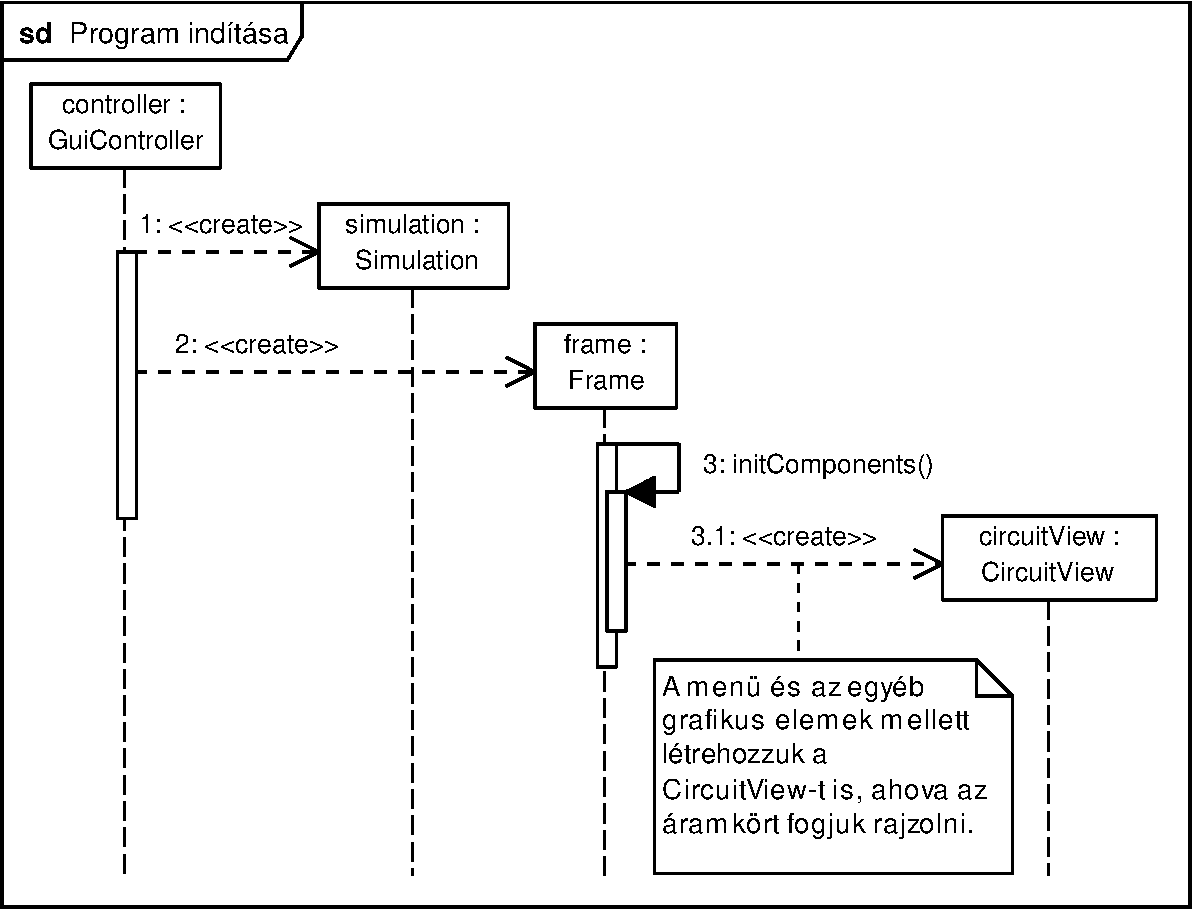
\includegraphics[width=17cm]{chapters/chapter11/pdfs/1_program_start.pdf}
\caption{Program indítása}
\label{fig:program_start}
\end{center}
\end{figure}

\begin{figure}[h]
\begin{center}
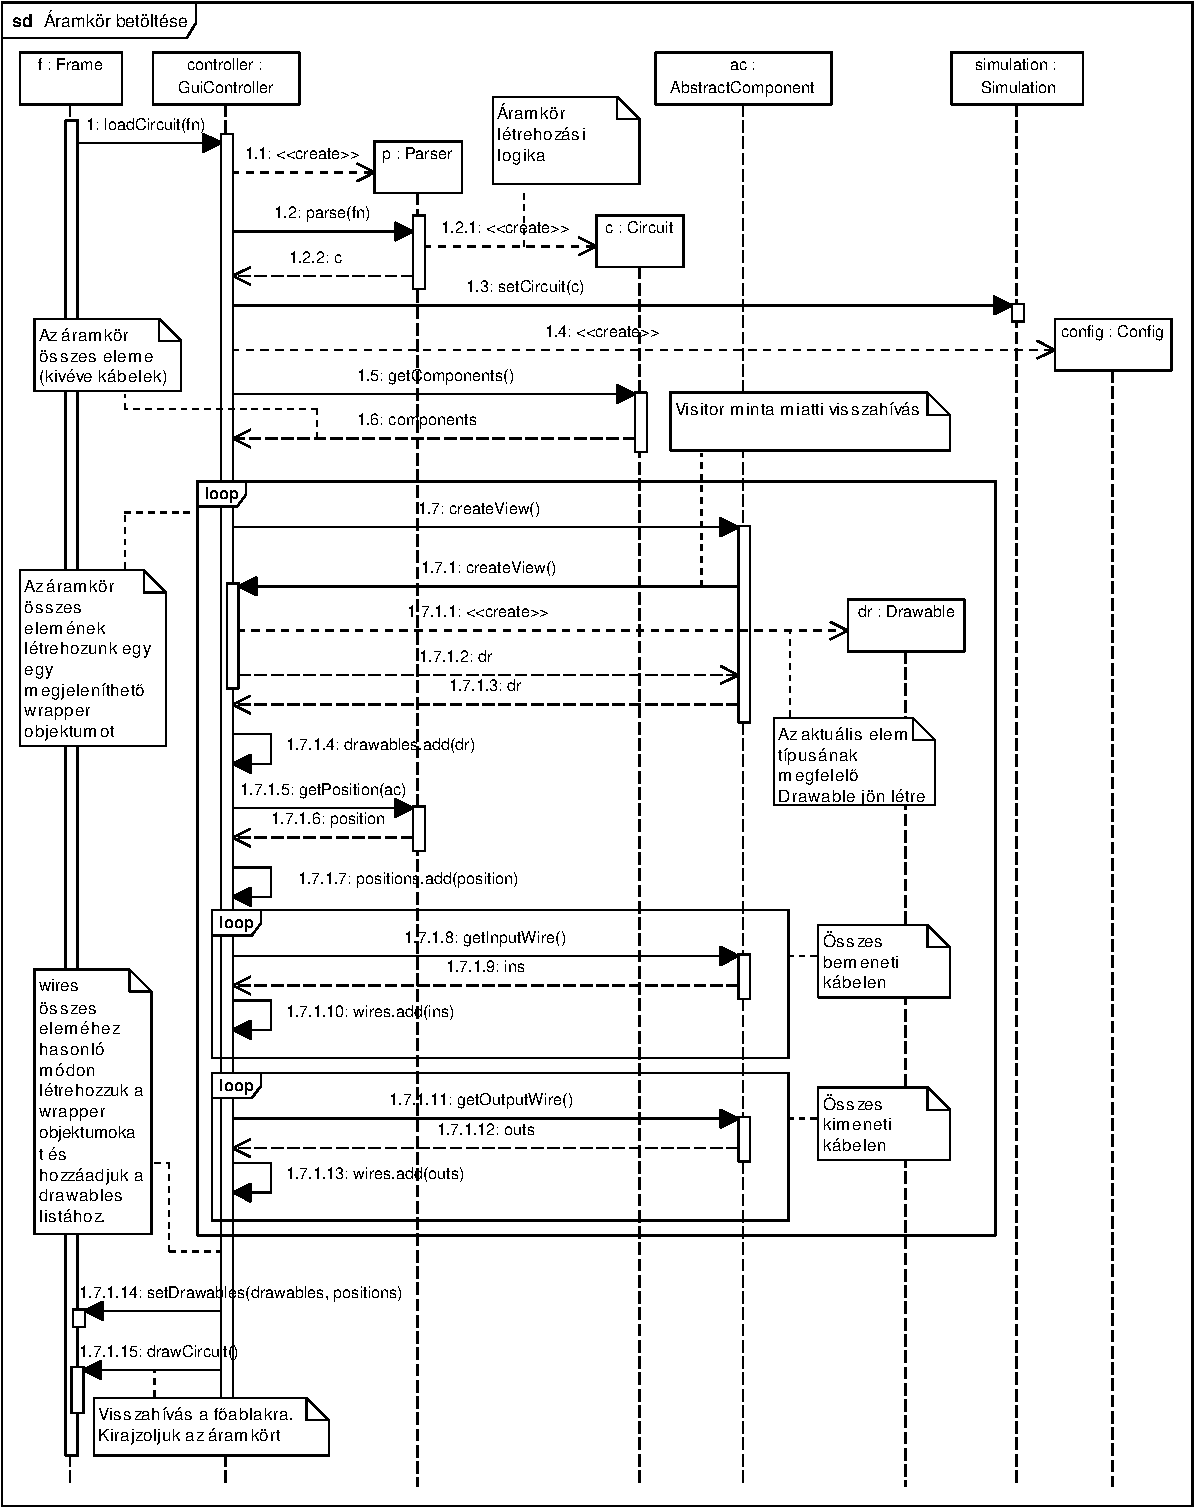
\includegraphics[width=17cm]{chapters/chapter11/pdfs/2_loadcircuit.pdf}
\caption{Áramkör betöltése}
\label{fig:loadcircuit}
\end{center}
\end{figure}

\begin{figure}[h]
\begin{center}
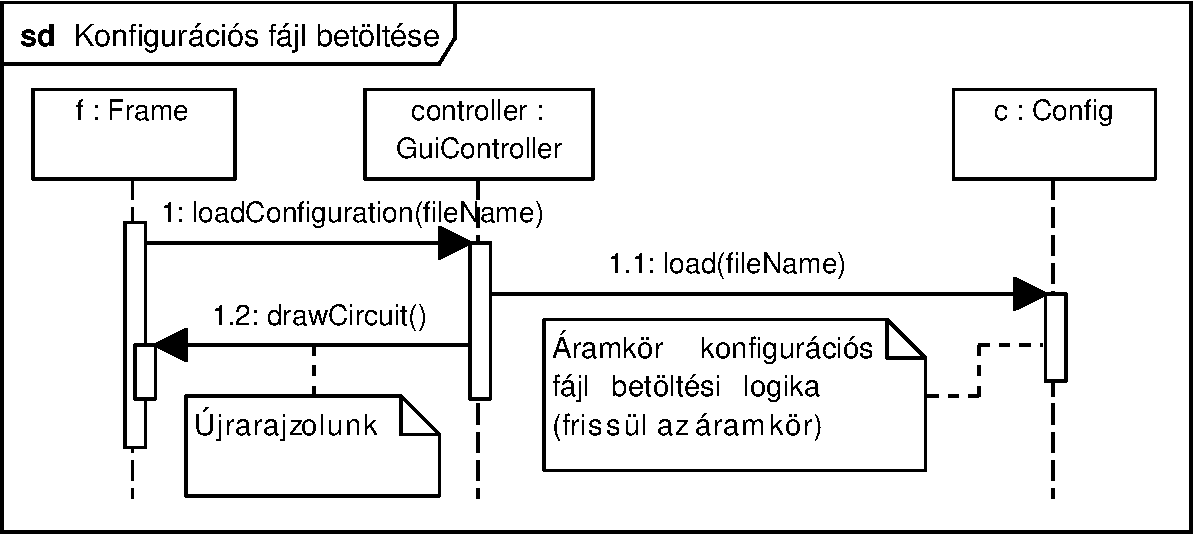
\includegraphics[width=17cm]{chapters/chapter11/pdfs/3_loadconfig.pdf}
\caption{Konfigurációs fájl betöltése}
\label{fig:loadconfig}
\end{center}
\end{figure}

\begin{figure}[h]
\begin{center}
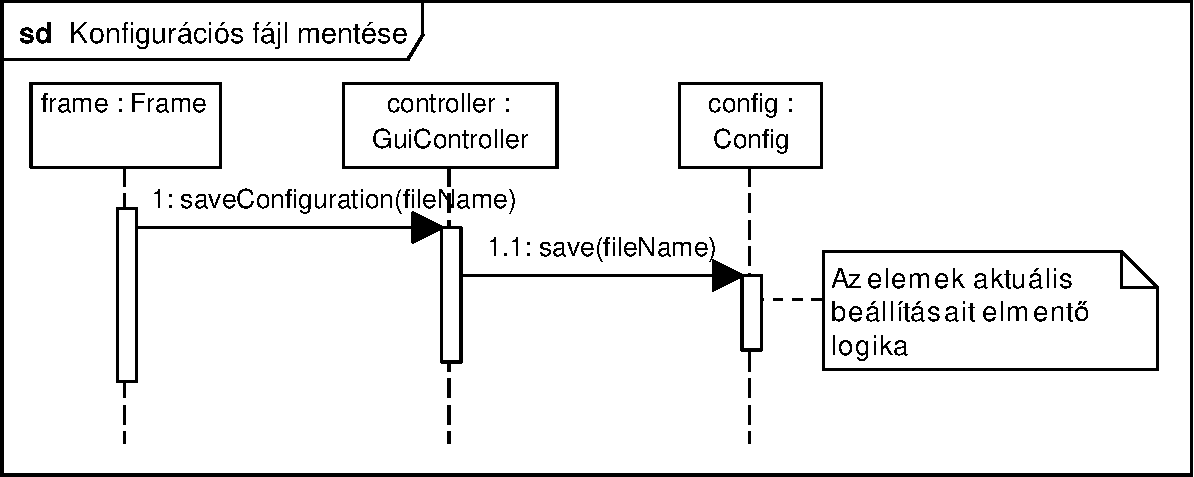
\includegraphics[width=17cm]{chapters/chapter11/pdfs/4_saveconfig.pdf}
\caption{Konfigurációs fájl mentése}
\label{fig:saveconfig}
\end{center}
\end{figure}

\begin{figure}[h]
\begin{center}
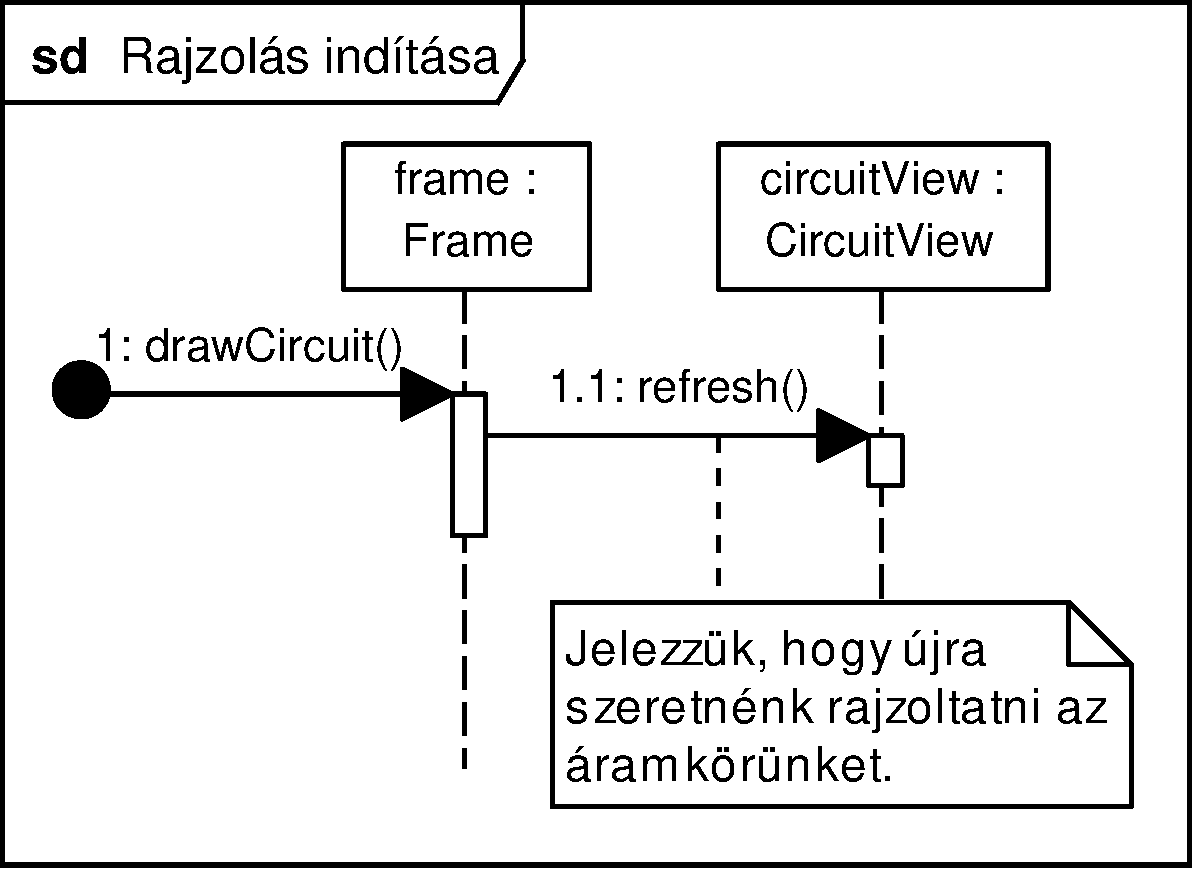
\includegraphics[width=10cm]{chapters/chapter11/pdfs/5_paint1.pdf}
\caption{Rajzolás indítása}
\label{fig:paint1}
\end{center}
\end{figure}

\begin{figure}[h]
\begin{center}
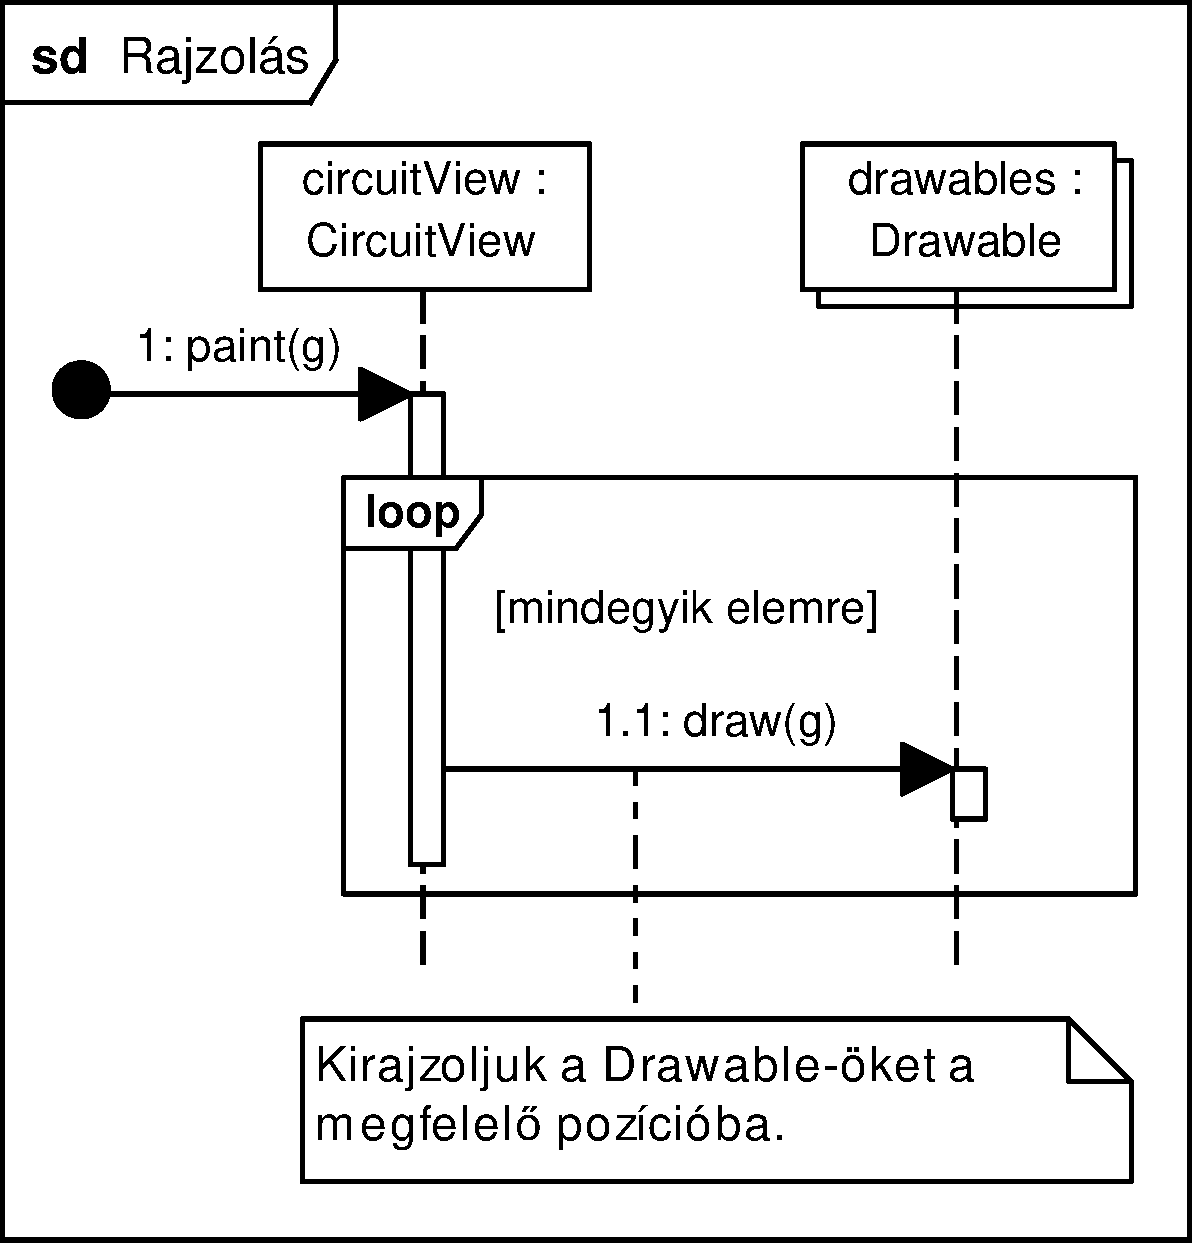
\includegraphics[width=10cm]{chapters/chapter11/pdfs/6_paint2.pdf}
\caption{Rajzolás}
\label{fig:paint2}
\end{center}
\end{figure}

\begin{figure}[h]
\begin{center}
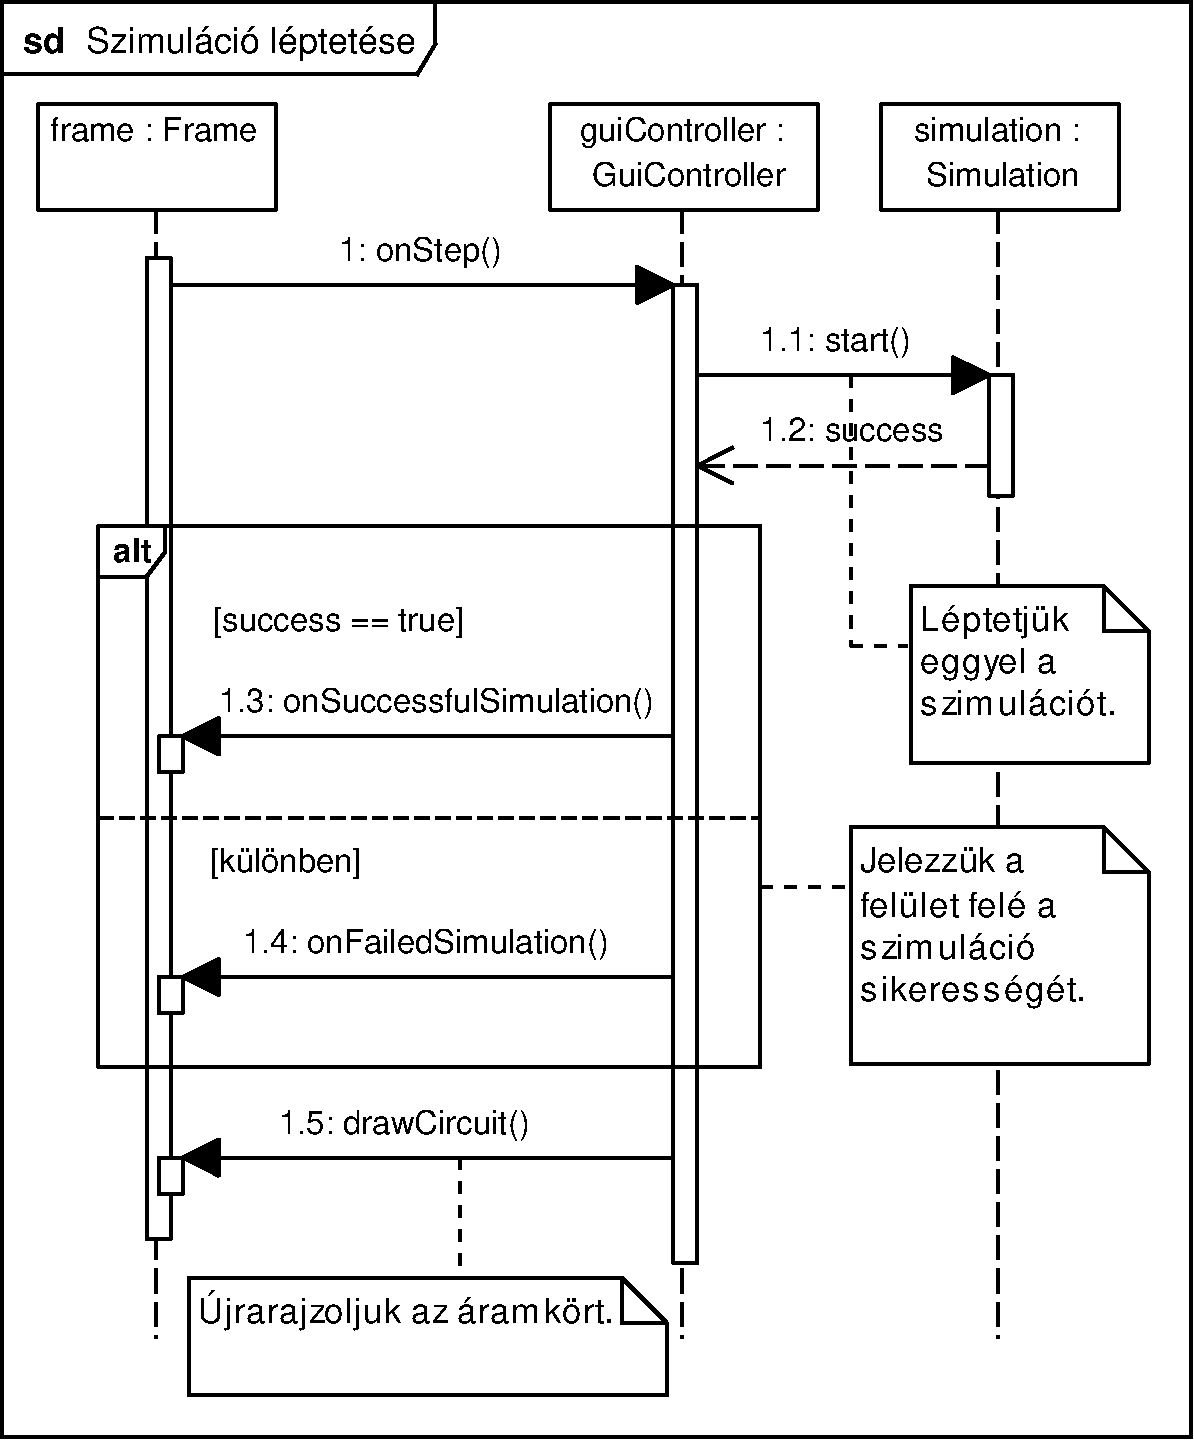
\includegraphics[width=15cm]{chapters/chapter11/pdfs/7_step.pdf}
\caption{Szimuláció léptetése}
\label{fig:step}
\end{center}
\end{figure}

\begin{figure}[h]
\begin{center}
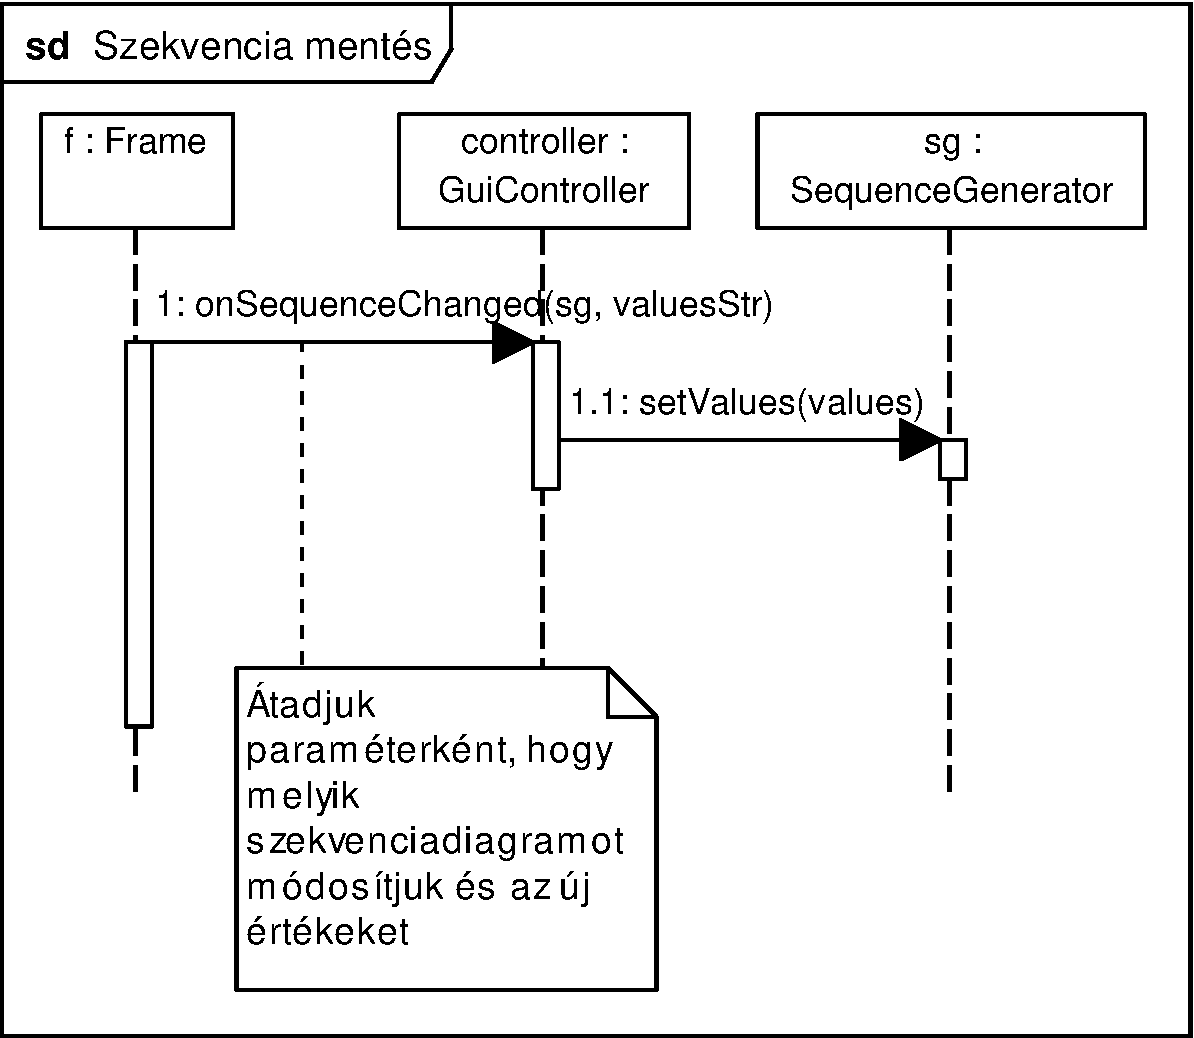
\includegraphics[width=10cm]{chapters/chapter11/pdfs/8_newsequence.pdf}
\caption{Szekvencia mentése}
\label{fig:newsequence}
\end{center}
\end{figure}

\begin{figure}[h]
\begin{center}
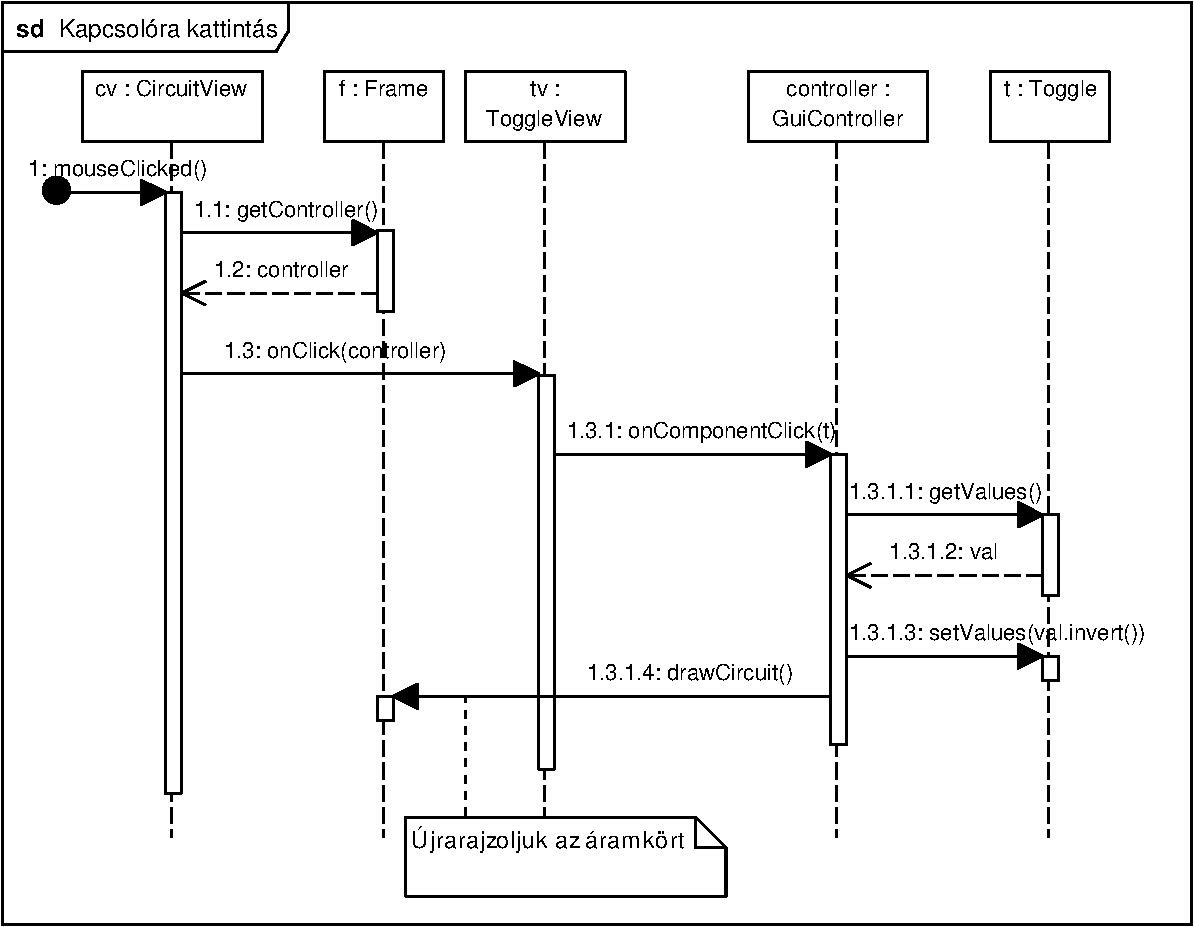
\includegraphics[width=17cm]{chapters/chapter11/pdfs/9_toggle.pdf}
\caption{Kapcsolóra kattintás}
\label{fig:toggle}
\end{center}
\end{figure}

\begin{figure}[h]
\begin{center}
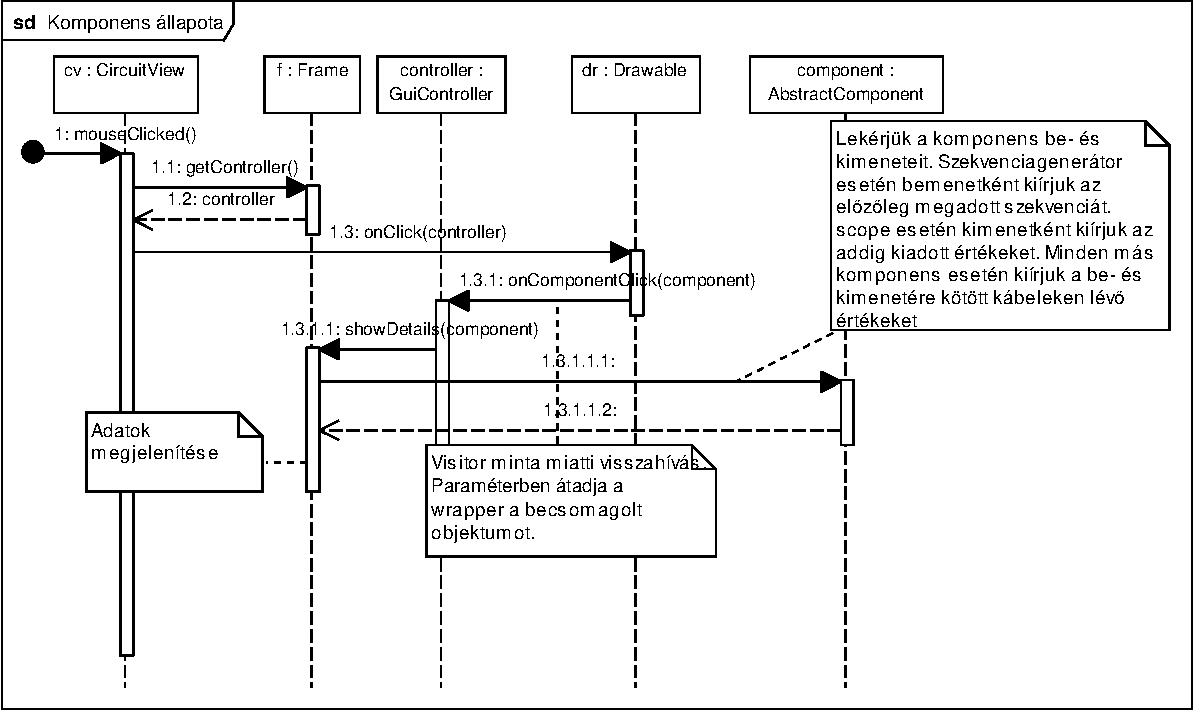
\includegraphics[width=17cm]{chapters/chapter11/pdfs/10_showcomponent.pdf}
\caption{Komponens állapotának kijelzése}
\label{fig:showcomponent}
\end{center}
\end{figure}

\begin{figure}[h]
\begin{center}
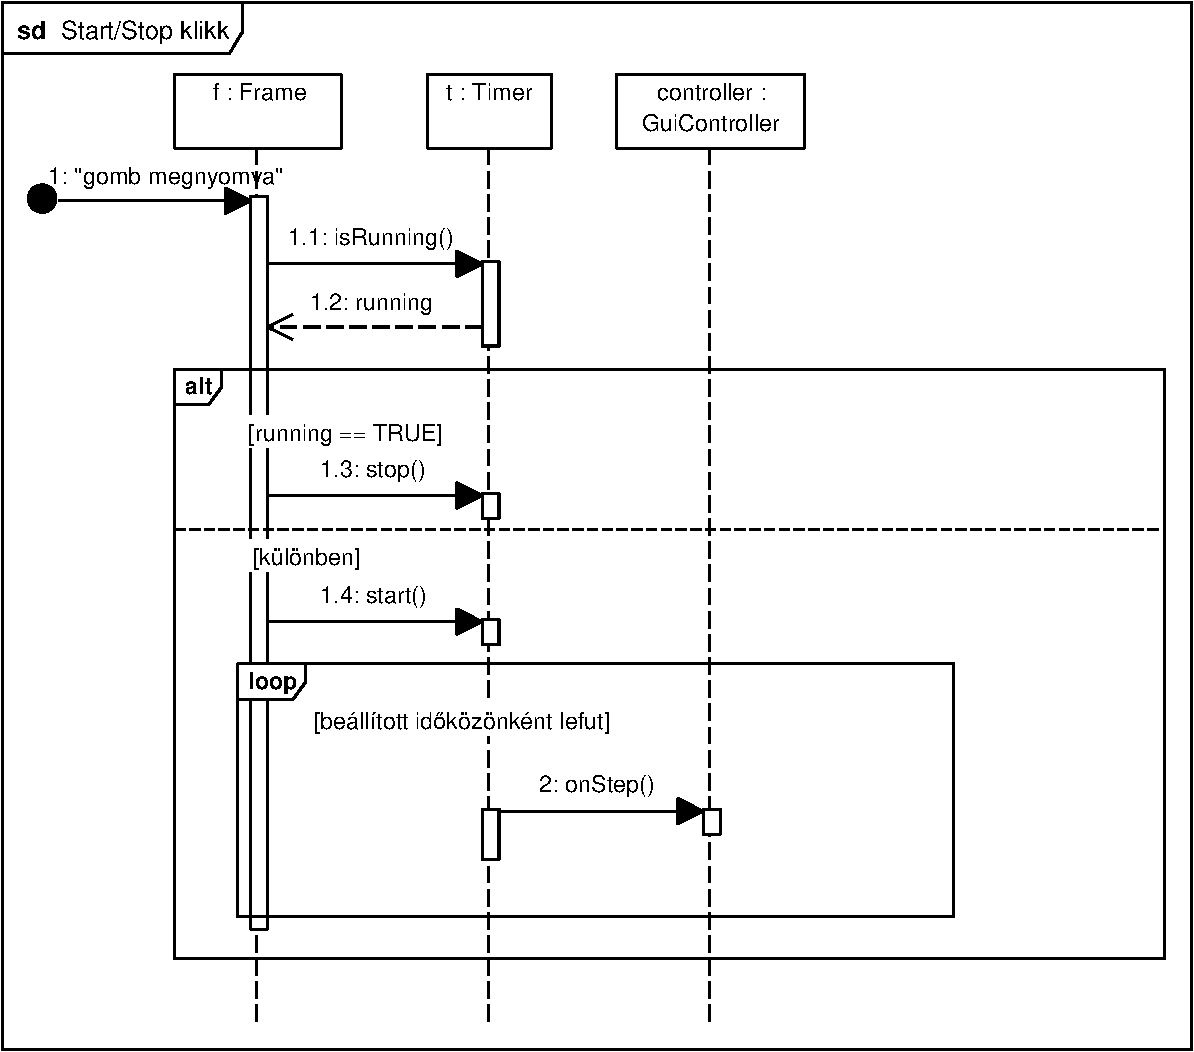
\includegraphics[width=17cm]{chapters/chapter11/pdfs/11_startstop.pdf}
\caption{Start/Stop klikk}
\label{fig:startstop}
\end{center}
\end{figure}

\begin{figure}[h]
\begin{center}
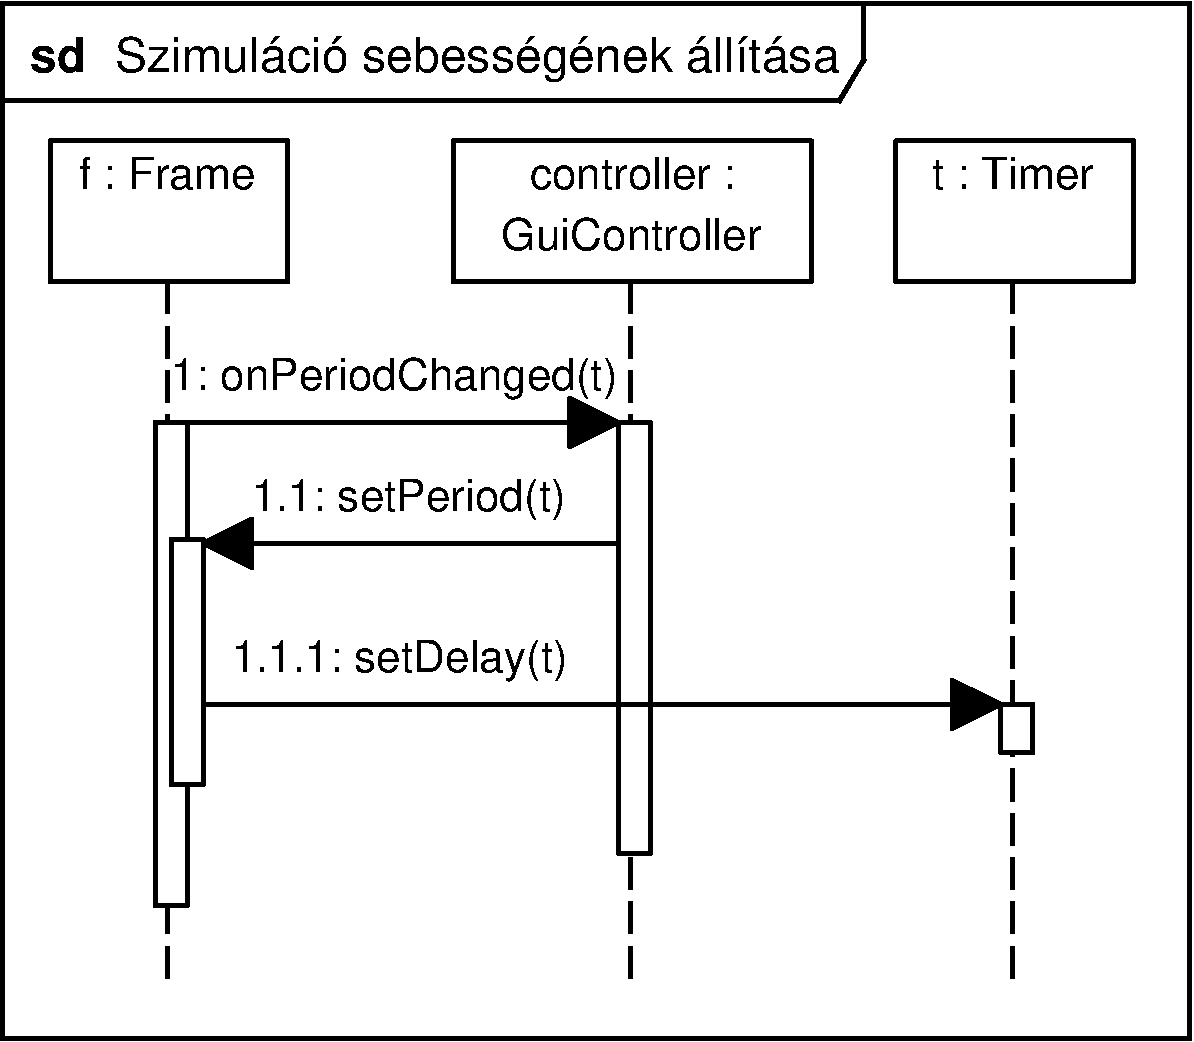
\includegraphics[width=6cm]{chapters/chapter11/pdfs/12_szimseb.pdf}
\caption{Szimuláció sebességének állítása}
\label{fig:szimseb}
\end{center}
\end{figure}